% =====================================================================
%  Does Multi-Paradigm Composition Improve NFR Classification?
%  Submission draft. Corrected after a full statistical audit; see
%  code/verify_paper.py, which recomputes every figure below.
% =====================================================================
\documentclass[11pt,a4paper]{article}

\usepackage[T1]{fontenc}
\usepackage[utf8]{inputenc}
\usepackage{mathptmx}
\usepackage{microtype}
\usepackage{amsmath,amssymb}
\usepackage{booktabs}
\usepackage{graphicx}
\usepackage{caption}
\usepackage{authblk}
\usepackage[a4paper,margin=2.4cm]{geometry}
\usepackage[hidelinks]{hyperref}

\captionsetup{font=small,labelfont=bf}

% float placement: the results section carries four floats in one subsection,
% so relax the defaults to keep each near its first citation
\renewcommand{\topfraction}{0.92}
\renewcommand{\bottomfraction}{0.75}
\renewcommand{\textfraction}{0.06}
\renewcommand{\floatpagefraction}{0.80}
\setcounter{topnumber}{3}
\setcounter{bottomnumber}{2}
\setcounter{totalnumber}{5}
\setlength{\parskip}{3pt}
\renewcommand{\arraystretch}{1.15}

\title{\bfseries Architectural Complexity in NFR Classification: Controlled\\
Ablations, Robustness Analyses, and a Six-Label Component Follow-Up}

\author[1]{Ahmad Nabot}
\author[2]{Shadi Nashwan}
\affil[1]{\small Al-Zaytoonah University of Jordan, Amman, Jordan \\ \texttt{a.nabot@zuj.edu.jo}}
\affil[2]{\small Middle East University, Amman, Jordan \\ \texttt{snashwan@meu.edu.jo}}
\date{}

\begin{document}
\maketitle

% =====================================================================
\begin{abstract}
\noindent
\textbf{Context.} Non-functional requirements (NFR) classifiers increasingly combine pre-trained encoders
with graph, relative-position, contrastive and meta-learning mechanisms. Model-level comparisons rarely
isolate the contribution of individual mechanisms or test whether conclusions depend on the label space.

\noindent
\textbf{Objectives.} We test whether four additions to a fine-tuned encoder produce a resolvable
macro-$F_1$ gain on a public NFR corpus, whether the conclusion survives documented protocol
sensitivities, and which components contribute when all six mapped quality labels are retained.

\noindent
\textbf{Methods.} The primary four-label experiment uses 1,667 requirements and five repetitions of
stratified five-fold cross-validation, giving 175 transformer fits. Robustness extensions examine source
shift, limited equal-trial-budget tuning, near-duplicate-grouped splitting and pair-aware contrastive
batching. A six-label sensitivity rebuilds the corpus at 1,719 requirements, and an exploratory
post-primary component follow-up reuses those frozen folds for four ablations, giving 453 fits in all.
Paired intervals use 4,000 record-level bootstrap resamples, conditional on the observed corpus.

\noindent
\textbf{Results.} Full reaches macro $F_1 = 0.8984$ against 0.8966 for encoder-only; removing a single
component changes macro $F_1$ by 0.0001--0.0051 and no 95\% interval admits a contribution above 0.015.
The protocol sensitivities establish no reliable aggregate advantage. The six-label task changes the
comparison: $0.8286 \pm 0.0113$ against $0.8038 \pm 0.0088$ ($\Delta = +0.0248$, 95\% CI
$[+0.0044, +0.0469]$). The component follow-up resolves two of four mechanisms, GCN removal costing
$+0.0225$ (Bonferroni 98.75\% CI $[+0.0023, +0.0474]$) and contrastive removal $+0.0207$
($[+0.0054, +0.0371]$). The four marginal effects sum to $+0.0671$ against a joint effect of $+0.0248$.

\noindent
\textbf{Conclusion.} Architectural value is conditional on the evaluated task. A simpler encoder remains
competitive under the four-label protocol, whereas the six-label follow-up identifies measurable GCN and
contrastive contributions. These are marginal removal effects local to this corpus and implementation,
not a decomposition of the endpoint difference, and the two restored labels hold only 34 and 18 records.

\medskip
\noindent\textbf{Keywords:} non-functional requirements; requirements classification; ablation study;
robustness analysis; class imbalance; task definition; sensitivity analysis; replication
\end{abstract}

\begin{center}
\fbox{\parbox{0.93\textwidth}{\small
\textbf{Scope of these results.} The findings hold for one corpus and one set of
hyperparameter settings. The corpus comprises 1{,}667 requirements in which a single class
holds 80.6\% of records, one collection supplies 64.2\%, and two of six ISO/IEC 25010
categories carry too few examples to evaluate. No hyperparameter optimisation was performed for the
primary controlled ablation, though a limited equal-trial-budget nested tuning sensitivity is reported
(Section~\ref{sec:protocolsens}), and no human baseline exists for this task. Sections~\ref{sec:threats} and \ref{sec:future} treat
each in turn.}}
\end{center}

\medskip

% =====================================================================
\section{Introduction}
\label{sec:intro}

Requirements classification assigns natural-language requirement statements to quality
categories, most commonly those of ISO/IEC 25010:2011~\cite{iso25010}. A point of terminology: the source datasets carry six quality labels that map onto
characteristics in that standard but are a subset of it, not the complete taxonomy. We write
``quality labels'' for what the corpora contain, retain the 2011 mapping because the source
annotations follow it, and note that the 2023 revision restructures several characteristics, so
a corpus annotated against it would not be directly comparable. Non-functional
requirements (NFRs) constrain how a system behaves rather than what it does, and their
early identification shapes architectural decisions whose later revision is
expensive~\cite{iso29148,chung2012}. Manual classification does not scale to industrial requirement volumes, and poorly elicited, documented
and managed requirements are a documented contributor to project failure~\cite{hussain2016}. Individual
quality attributes compound the difficulty: security requirements in particular have long been argued to
be under-specified in practice~\cite{firesmith2003}.

Automation has followed the trajectory of natural language processing more broadly. Early
work applied classical machine learning over engineered features~\cite{casamayor2010,slankas2013,abad2017}. Deep architectures removed the feature-engineering step~\cite{haque2019,rahimi2021}. Transfer learning from pre-trained transformers established the current state of the art~\cite{hey2020,subahi2023}. Recent
proposals compose several paradigms at once, adding graph neural networks over domain
ontologies~\cite{liu2022,song2021}, extended-context
mechanisms~\cite{dai2019}, contrastive objectives~\cite{khosla2020}, and meta-learning
for cross-domain adaptation~\cite{finn2017,chen2025}.

The rationale for composition is intuitive: each paradigm addresses a failure mode the
others share. A token-sequence encoder cannot represent explicit relations among quality attributes. A graph network generalises poorly where training data is thin, and neither handles requirements exceeding the encoder's context window. Composing them should yield
a classifier stronger than any single mechanism.

That expectation is seldom tested. Papers proposing composed architectures typically
report a headline comparison against published baselines evaluated on different corpora
under different splits, which cannot separate architectural contribution from
experimental variance. Dell'Anna et al.~\cite{dellanna2023} document how often classifier
evaluations in software engineering omit multi-seed estimation, effect sizes, and
confidence intervals, and propose the ECSER pipeline as a remedy. Component-level
ablation, which removes one mechanism at a time while holding data, folds, and
hyperparameters fixed, is the control that isolates architectural contribution, and it
is largely absent from this literature.

This paper reports such a control and its outcome, which is negative. We address three
research questions.

\textbf{RQ1.} Does each paradigm in a composed NFR classifier contribute measurably to
classification performance when data, folds, seeds, and hyperparameters are held fixed?

\textbf{RQ2.} If not, what magnitude of contribution can the evaluation exclude, and how
does the composed architecture compare against a bare fine-tuned encoder, an independently
developed transfer-learning baseline, and a classical pipeline evaluated on the same folds?

\textbf{RQ3.} What accounts for the variation in per-category performance that architecture
does not, and how much of it is attributable to the volume of labelled data per category?

RQ1 and RQ2 are answered in Sections~\ref{sec:ablation} and \ref{sec:norbert}, RQ3 in
Section~\ref{sec:support}. We implement
MAGNET-NFR with every component independently ablatable, and evaluate six architectural
configurations, an independently developed transfer-learning baseline, and a classical
pipeline on identical cross-validation folds, a total of 175 transformer training runs
(Sections~\ref{sec:architecture} and \ref{sec:design}). No component contributes
measurably. We quantify what the design excludes rather than resting on non-significance. Confidence intervals on every ablation are narrow enough to rule out single-component contributions above 0.015 macro $F_1$, which makes this a bounded null rather than
a failure to reject (Section~\ref{sec:ablation}).

We then show that per-category performance is governed by category rather than by method,
in a ratio of 91.5\% of variance to 1.5\%, and isolate class support as one
causal driver through a matched-support experiment. Capping the majority category's training data at the minority category's support costs 0.083 $F_1$, or 43\% of the
gap between them (Section~\ref{sec:support}). The remaining 57\% remains unexplained by training-set size, and we test and reject the obvious explanation for it. Alongside these
results we assemble and release a corpus of 1,667 requirements with per-record provenance
and a full deduplication audit that recovers a sub-source breakdown showing seven
documented collections, one supplying 64.2\% of records and another proving 84\%
internally duplicated
(Section~\ref{sec:corpus}). The code, fold assignments, and all prediction sets are
released with a script that recomputes every number reported here
(Section~\ref{sec:reproducibility}).

The paper proceeds as follows. Section~\ref{sec:related} reviews the task, the corpora the
field depends on, the methods proposed for it, and the wider literature on re-examining
architectural progress under controlled comparison, from which this study takes its design.
Section~\ref{sec:methods} describes the corpus, its provenance in Table~\ref{tab:provenance} and its composition in
Figure~\ref{fig:corpus}, the architecture and its ablation points in
Figure~\ref{fig:architecture}, the settings in Table~\ref{tab:hyper}, and the
cross-validation design and statistical procedure.

Section~\ref{sec:results} reports the experiments, including the source-aware evaluation of Section~\ref{sec:loso}. Table~\ref{tab:results} and Figure~\ref{fig:effects} give the headline comparison across
all eight configurations with interval estimates, and Table~\ref{tab:equiv} the equivalence
tests against a declared smallest effect of interest. Table~\ref{tab:percat} gives per-category performance;
Figure~\ref{fig:support} decomposes the variance between category and method.
Table~\ref{tab:matched} and Figure~\ref{fig:matched} report the matched-support experiment
that separates class support from category identity. Figure~\ref{fig:convergence} shows training dynamics. Section~\ref{sec:discussion} interprets these results and states what
follows for research practice and for practitioners. Section~\ref{sec:threats} addresses
threats to validity, Section~\ref{sec:future} sets out the limitations and the work they
motivate, and Section~\ref{sec:conclusion} concludes.

% =====================================================================
\section{Related Work}
\label{sec:related}

This section covers what makes NFR classification difficult
(Section~\ref{sec:rw-task}), the corpora the field relies on and how their properties bound
any experiment conducted on them (Section~\ref{sec:rw-corpora}), the methods proposed for the
task (Sections~\ref{sec:rw-methods} and \ref{sec:rw-composed}), the controlled
re-examinations from which this study takes its design (Section~\ref{sec:rw-scrutiny}), and
evaluation methodology, closing with the gap the preceding material leaves
(Section~\ref{sec:rw-eval}).

\subsection{The classification task and why it resists automation}
\label{sec:rw-task}

An NFR constrains the quality or operational characteristics of a system rather than
describing a function it performs~\cite{glinz2007}. Chung et al.~\cite{chung2000}
formalised quality attributes as softgoals satisficed by degree, and showed that
architectural decisions typically affect several simultaneously. Two consequences follow
for automated classification, and both recur in our results.

The categories are not disjoint. A requirement stipulating encrypted replication to a
standby server within a fixed interval concerns security, reliability and performance at
once, so a single-label formulation misrepresents it whatever the classifier. Nor is the
ISO/IEC 25010 partition the one practitioners use when evaluating a working system.
Althunibat~\cite{althunibat2025} assesses a deployed government application against three
quality aspects, grouping reliability with ease of use under performance quality, where the
standard treats reliability and usability as distinct characteristics. The regrouping is not
an error but reflects which distinctions matter for a system in service rather than a
specification, so a classifier trained on the standard's partition learns one defensible
carving among several. Cleland-Huang et al.~\cite{clelandhuang2007} confronted this in an early and influential
automated NFR classifier built on indicator terms mined from a training set. Their
evaluation used thirty requirements specifications written as term projects by graduate
students, together with one industrial document, and that student-project collection became
the PROMISE NFR dataset. The provenance is worth recording, since a benchmark assembled from
coursework carries different properties from one drawn from industrial practice, and the
field has relied on it for close to two decades. Their framing, that categories
are identified by characteristic vocabulary, has proved durable. We find in Section~\ref{sec:results} that a bag-of-bigrams model still recovers most of the achievable
performance.

The categories are also unevenly represented in practice. Security and performance
requirements are written frequently and in standardised language. Maintainability and portability requirements are written rarely and in prose that varies more between
organisations. Studies reporting per-category results, including Kurtanović and
Maalej~\cite{kurtanovic2017} and Dalpiaz et al.~\cite{dalpiaz2019}, evaluate on corpora in
which the categories differ greatly in frequency. What has not been done is
to separate the contribution of labelled-data volume from that of category identity, since
the two are confounded in every published corpus. That separation is the experiment we
report in Section~\ref{sec:support}.

\subsection{The corpora the field relies on}
\label{sec:rw-corpora}

Most studies cited in this section evaluate on one of a small number of shared
collections, and their properties propagate into every result built on them. The PROMISE NFR
dataset~\cite{clelandhuang2007} comprises 625 labelled requirements, small by contemporary
standards, and remains the most frequently cited benchmark in this literature. PURE~\cite{ferrari2017} is a collection of public
requirements documents assembled to support natural-language processing research on
requirements. SecReq~\cite{knauss2011} was assembled to study security requirements and is
correspondingly skewed toward that category. Redistributed aggregations combine these with
further collections, and as Section~\ref{sec:corpus} shows, the composition of such an
aggregation is not always evident from its filename.

Three properties follow. The corpora are small by contemporary standards, so estimates carry
wide intervals. They are severely imbalanced, and imbalance depresses minority-class recall
while leaving aggregate accuracy largely intact~\cite{he2009}, which makes accuracy a
misleading headline metric here. And PROMISE and its extensions recur often enough that
agreement between papers is weaker evidence than it appears, since the same annotation
decisions and imbalance are inherited each time. Six of the eleven studies surveyed in Section~\ref{sec:rw-eval} evaluate on PROMISE or a derivative, though recent work has
begun to move away: Li and Nong~\cite{li2022} built an expanded corpus because PROMISE was
inadequate, and Alhaizaey et al.~\cite{alhaizaey2025} label over ten thousand user stories.
Our own corpus, drawn from an aggregation of these and related collections, is subject to all
three limitations. Section~\ref{sec:corpus} quantifies them rather than passing over them, and
recovers the sub-source composition that the aggregation documents but does not advertise.

\subsection{From engineered features to pre-trained encoders}
\label{sec:rw-methods}

Classical pipelines over engineered features established the task: semi-supervised labelling
reduction~\cite{casamayor2010}, extraction from heterogeneous documents~\cite{slankas2013}, and the
finding that preprocessing choices move performance substantially~\cite{abad2017}. Kurtanović and
Maalej~\cite{kurtanovic2017} applied support vector machines to lexical and syntactic features,
illustrating a pattern that recurs below: strong classical baselines exist here and later neural work has
often not compared against them directly. All share a structural limitation, in that a human decides in
advance which features matter.

Deep architectures removed that constraint, through convolutional
networks~\cite{winkler2016,haque2019}, attention-augmented LSTM ensembles~\cite{rahimi2021}, and
feed-forward and convolutional multi-class classifiers~\cite{baker2019}. Li and Nong~\cite{li2022}
proposed a BERT and Bi-LSTM architecture, constructing an expanded corpus expressly because PROMISE was
too small to support their evaluation.

Two comparisons bear directly on our results, both concerning the classical baseline. Canedo
and Mendes~\cite{canedo2020} found TF-IDF with logistic regression best among four classifiers
and three feature schemes on PROMISE-exp, and record a gap we reproduce: $F$ = 0.91 for the
binary decision against 0.74 for NFR sub-classification. Rahman et al.~\cite{rahman2023}
evaluated fifteen algorithms on the same collection and likewise found a linear support vector
classifier over TF-IDF best. The classical pipeline is not a straw baseline here, and any
claim of neural improvement must clear it. Recurrent models handle long-range dependencies poorly, a limitation
self-attention was designed to remove~\cite{vaswani2017}.

Transfer learning followed. BERT~\cite{devlin2019} established the fine-tuning paradigm,
RoBERTa~\cite{liu2019roberta} improved its pre-training recipe, and distilled
variants~\cite{sanh2019} reduced the cost; we use one such variant. Hey et al.~\cite{hey2020}
adapted this to requirements with NoRBERT, reporting $F_1 = 0.87$ on PROMISE with degradation
on unseen projects, and Subahi~\cite{subahi2023} reported gains from domain-adaptive
pre-training. Shafikuzzaman et al.~\cite{shafikuzzaman2025} found zero-shot and few-shot
approaches below supervised counterparts, indicating labelled data remains the binding
constraint. We adopt NoRBERT as our reference baseline and re-train it on our folds.

\subsection{Composed architectures}
\label{sec:rw-composed}

Graph convolutional networks propagate information along relational structure, letting a model consume
explicit domain knowledge rather than infer it distributionally~\cite{liu2022,song2021}; applied to
requirements, the appeal is that quality attributes stand in relations an encoder would otherwise infer
from co-occurrence. Transformer-XL extends the effective context window through segment-level
recurrence~\cite{dai2019}, supervised contrastive learning tightens intra-class geometry before
classification~\cite{khosla2020}, and model-agnostic meta-learning adapts across tasks from few
examples~\cite{finn2017}, which Saleem et al.~\cite{saleem2025} apply to requirements and Chen et
al.~\cite{chen2025} to adaptation under changed conditions outside this field.

Each mechanism is well motivated in isolation, and each addresses a limitation the others
share. The premise of composition is that these limitations are independent, so that
addressing them jointly yields a classifier stronger than any single mechanism. That premise
is what we test.

\subsection{Architectural progress under controlled comparison}
\label{sec:rw-scrutiny}

The question we ask has an established answer elsewhere in software engineering, and a
consistent one in adjacent fields, which together motivate asking it of NFR classification.

Within software engineering, Lessmann et al.~\cite{lessmann2008} benchmarked 22 classifiers
across ten defect-prediction datasets and found no significant differences among the top 17,
concluding that algorithm choice may matter less than assumed. That result frames what
follows: the possibility is not novel in this discipline, and the open question is how far it
extends and what controls establish it.

Two re-examinations outside software engineering supply the controls. Melis et
al.~\cite{melis2018} re-evaluated a succession of neural language-model architectures under
large-scale black-box hyperparameter tuning and found that properly regularised LSTMs
outperformed the models reported to have superseded them. Dacrema et
al.~\cite{dacrema2019} examined eighteen neural recommendation methods presented at top-level conferences. Only seven could be reproduced with reasonable effort, and six of
those seven were often outperformed by simple heuristic baselines. Their companion
study~\cite{dacrema2021} reports that eleven of twelve reproducible neural approaches were
beaten by conceptually simple methods. The reproducibility failure rate in that work is as
instructive as the performance comparison. Lipton and Steinhardt~\cite{lipton2019}
catalogue the practices that produce these patterns, among them the conflation of
architectural change with tuning effort and the absence of ablation.

Our contribution is therefore not to introduce controlled comparison to software engineering
but to bring a control these studies did not use, component-level ablation under fixed data
and hyperparameters, to a task where composed architectures have accumulated rapidly.
Requirements classification is a good candidate, because the corpora are small and heavily reused,
and the field's own methodological guidance~\cite{dellanna2023} identifies evaluation
practice as a weakness.

\subsection{Evaluation methodology and the gap it leaves}
\label{sec:rw-eval}

Dell'Anna et al.~\cite{dellanna2023} found frequent omission of multi-seed estimation, effect sizes and
confidence intervals in software-engineering classifier evaluation; their ECSER pipeline prescribes each.
Ralph et al.~\cite{ralph2020} set out comparable empirical standards, and Wohlin et al.~\cite{wohlin2012}
supply the validity taxonomy used in Section~\ref{sec:threats}.

An older statistical literature bears directly on our choices.
Dietterich~\cite{dietterich1998} recommended McNemar's test for paired comparison on a single
held-out set while warning against tests that treat resampled evaluations as independent.
Demšar~\cite{demsar2006} established the Friedman test as the standard for comparing multiple
classifiers and noted its low power with few blocks, which is why we report it descriptively.
Reimers and Gurevych~\cite{reimers2017} showed single-run comparisons to be unreliable and
recommended reporting score distributions. Section~\ref{sec:stats} explains why these
recommendations, applied to repeated cross-validation on an imbalanced corpus, lead us to a
record-level bootstrap rather than McNemar's test.

\medskip
\noindent
Taken together, the preceding subsections identify a gap that is methodological rather than
technical. Two secondary studies already exist: Iipinge et al.~\cite{iipinge2023} screened 66 studies and
found supervised learning with ten-fold cross-validation dominant, and Kaur and
Kaur~\cite{kaur2024} mapped 60 and found transfer learning most accurate. We do not duplicate
either.



Across an illustrative sample of eleven studies, assembled by following citations rather than
systematic search, ten report no component-level ablation and the eleventh a partial one, while
corpora and protocols differ enough that the figures are not mutually comparable. The field has
accumulated architectural claims whose individual contributions are unmeasured. This study
addresses that for one composition and releases folds on which later methods can be evaluated
identically.

% =====================================================================
\section{Methods}
\label{sec:methods}

Answering RQ1 and RQ2 requires an experiment in which the only thing varying between conditions is the presence of an architectural component. That is harder here than it sounds, because the available corpora are small, severely imbalanced and of uncertain composition, and because the natural tests for paired classifier comparison are the wrong ones for the metric carrying the claim. We take those problems in turn: the corpus (Section~\ref{sec:corpus}), the architecture and its cut points (Section~\ref{sec:architecture}), the design (Section~\ref{sec:design}), the inferential procedure (Section~\ref{sec:stats}) and what we release (Section~\ref{sec:reproducibility}).

\subsection{Corpus construction}
\label{sec:corpus}

We assembled the corpus from publicly available, previously labelled requirements
datasets rather than annotating from scratch. Two sources contributed usable records: a
curated Mendeley FR/NFR collection, and a consolidated aggregation of the PROMISE, PURE,
and SecReq corpora. A third candidate file was excluded after inspection because it
carries only a binary functional/non-functional flag with no NFR sub-category.

Labels are inherited from the source corpora; we did not re-annotate and make no
inter-annotator agreement claim. We normalised label spellings, discarded functional
requirements, and removed records whose labels lie outside the standard, principally
scalability, legal and operational codes from the PROMISE-derived data.

Selecting the label column requires care. Both source files contain two label-bearing columns, a binary functional/non-functional flag and an NFR sub-category. Matching on
column name selects the binary flag and discards every NFR in the file. Our construction
script therefore scores each candidate column by the number of values that resolve to an
ISO/IEC 25010 category and selects the highest-scoring column. We record this because the
failure is silent: it yields an empty corpus rather than an error.

\paragraph{Deduplication and effective source contribution.}
We deduplicated on a punctuation- and case-insensitive fingerprint of the requirement
text. Table~\ref{tab:provenance} reports the full pipeline per source, which is necessary
to interpret what the corpus contains.

\begin{table}[htbp]
\centering
\caption{Corpus provenance. The aggregation file records the originating collection of
each requirement in a \texttt{Dataset\_Name} field, which we recover and trace through
deduplication and scope reduction. \textbf{Raw} counts rows carrying usable requirement
text, which is why the aggregation contributes 3{,}471 of its 3{,}482 rows.
\textbf{Unique} counts distinct requirement texts within each collection. These do not sum to the 1{,}719 total because deduplication is applied globally, so a text appearing in two
collections is counted once in the total and once in each collection's own figure.
\textbf{Final} counts records surviving into the evaluated corpus after global
deduplication and the scope reduction described below.}
\label{tab:provenance}
\small
\setlength{\tabcolsep}{5pt}
\begin{tabular}{@{}lrrrr@{}}
\toprule
\textbf{Source file and documented collection} & \textbf{Raw} & \textbf{NFR} & \textbf{Unique} & \textbf{Final}\\
\midrule
\multicolumn{5}{@{}l@{}}{\emph{PROMISE / PURE / SecReq aggregation}}\\
\quad PURE\_and\_others & 1{,}083 & 1{,}083 & 1{,}082 & 1{,}071 \hfill (64.2\%)\\
\quad software\_requirements\_extended & 977 & 257 & 256 & 237 \hfill (14.2\%)\\
\quad promise\_exp & 969 & 411 & 409 & 165 \hfill (9.9\%)\\
\quad requirements\_MoSCoW & 108 & 108 & 108 & 108 \hfill (6.5\%)\\
\quad SecReq Customer Premises Network & 210 & 77 & 60 & 27 \hfill (1.6\%)\\
\quad SecReq Common Electronic Purse & 124 & 88 & 88 & 2 \hfill (0.1\%)\\
\addlinespace
\multicolumn{5}{@{}l@{}}{\emph{Curated Mendeley collection}}\\
\quad Complete\_Dataset sheet & 1{,}145 & 406 & 65 & 57 \hfill (3.4\%)\\
\midrule
\textbf{Total} & \textbf{4{,}616} & \textbf{2{,}430} & \textbf{1{,}719} & \textbf{1{,}667}\\
\bottomrule
\end{tabular}
\setlength{\tabcolsep}{6pt}
\end{table}

Table~\ref{tab:provenance} corrects an impression the two source files would otherwise
give. The aggregation is not a single corpus but a compilation of six documented
collections, which together with the Mendeley set makes seven contributing sources. Read
down the final column, however, the contribution is heavily concentrated: one collection
supplies 64.2\% of the evaluated records and the three smallest supply 5.1\% between them.
Results should be read as pertaining to this mixture, weighted as it is, rather than to any
single named corpus. In particular, the PROMISE-derived portion contributes 9.9\%, so this
is not principally a PROMISE study despite PROMISE being the benchmark most often cited in
this literature.

The dominant collection requires separate comment, because its composition explains a
property that would otherwise look like a general feature of NFR data. All 1,071 records from
\texttt{PURE\_and\_others} carry the Security label and the collection contributes nothing
else, so those records constitute 79.7\% of the 1{,}343 Security instances. The class
imbalance in Figure~\ref{fig:corpus} is therefore substantially an artefact of merging one
security-specific collection into the aggregation, and since the majority-class floor derived
from it governs every accuracy figure in Section~\ref{sec:results}, a reader is entitled to
know its origin.

This raises the possibility that Security's strong performance is a source effect rather than
a category effect. We tested it. Security recall for the full model, computed by originating
collection over five repeats, is 0.987 for \texttt{PURE\_and\_others} against 0.970 for the
remaining collections weighted by support, with individual collections between 0.939 and
1.000. The source effect of roughly 0.017 is an order of magnitude below the 0.171 spread
across categories, so the category effect of Section~\ref{sec:support} survives the
confound.

Two sources lose a large fraction of records to internal duplication. The Mendeley
collection is the extreme case, its 406 NFR records reducing to 65 distinct texts, an 84.0\%
rate, leaving 57 records after scope reduction. A reader counting rows in the published files
would otherwise overestimate the evidence available.

Exact deduplication does not catch near-duplicates. Using character 3--5-gram cosine
similarity, 138 records (8.3\%) have a neighbour at 0.90 or above, and 79\% of those pairs
span different folds. Templated requirements therefore cross the fold boundary, so absolute figures should be read
as upper bounds. Whether this inflates all configurations equally cannot be assumed, since architectures could exploit
templated phrasing to different degrees and the contrasts we interpret are thousandths of macro $F_1$. We
therefore construct a second set of folds in which every connected near-duplicate component is assigned
wholly to one outer fold, reducing pair crossings to zero in every repeat, and report the resulting
comparison in Section~\ref{sec:protocolsens}. Cross-source overlap is nil. One requirement text carries two different labels within the
aggregation, which we note in Section~\ref{sec:threats}. Because cross-source overlap is nil, no label conflict arises between the two files.

\paragraph{Class distribution and scope reduction.}
The resulting distribution is severely imbalanced. Figure~\ref{fig:corpus} plots record
counts and category shares.

\begin{figure}[htbp]
\centering
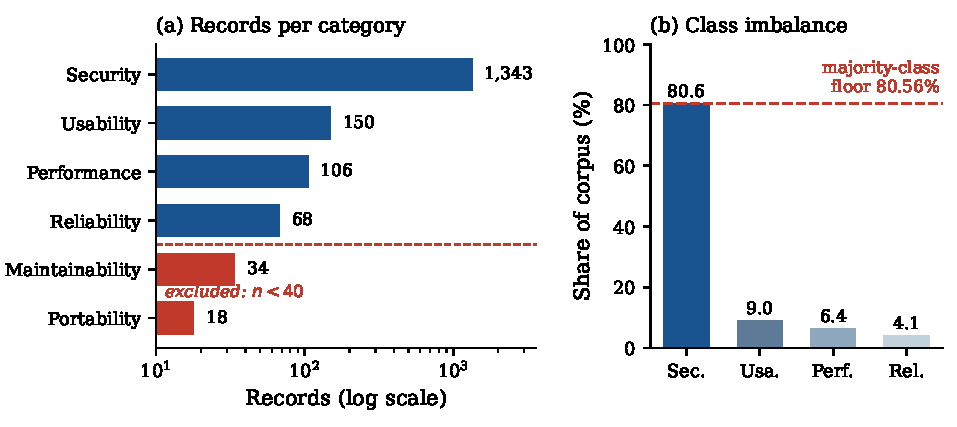
\includegraphics[width=\textwidth]{figures/fig_corpus.pdf}
\caption{Corpus composition after deduplication. (a) Record counts by ISO/IEC 25010
category on a logarithmic scale. Categories below the 40-record threshold (red) cannot support
a per-category $F_1$ with a usable confidence interval and are excluded. (b) Share of the
1{,}667 evaluated records by category, against the 80.56\% majority-class floor.}
\label{fig:corpus}
\end{figure}

Figure~\ref{fig:corpus}(a) shows a distribution spanning nearly two orders of magnitude,
from 1{,}343 Security records to 18 for Portability. Maintainability (34 records) and
Portability (18) fall below the threshold at which a per-category $F_1$ carries a usable
confidence interval, and we exclude them. The threshold is empirical: simulating bootstrap intervals at the minority-class error rate,
the 95\% half-width is 0.131 at $n = 34$ against 0.092 at $n = 68$, so at $n = 34$ a
per-category $F_1$ could not be distinguished from values a quarter of the scale apart. This is a data-availability
constraint rather than a design choice. It leaves four categories and 1{,}667 records
(Figure~\ref{fig:corpus}).



The distribution carries three consequences that govern every subsequent result.
First, Security accounts for 80.56\% of the evaluated corpus, so a classifier predicting
Security unconditionally achieves 80.56\% accuracy while learning nothing; accuracy figures
must be read as margins above that floor rather than above zero, and macro $F_1$, which
weights the three minority categories equally with Security, carries the
substantive claim throughout. Second, the support range is close to twenty-to-one between
the largest and smallest evaluated category, which is what makes the per-category analysis
of Section~\ref{sec:support} informative: the corpus contains a natural gradient in
labelled-data volume that we can exploit rather than merely regret. Third, the two excluded
categories are not marginal omissions but a third of the taxonomy, so results here speak to
four ISO/IEC 25010 categories and not to NFR classification in full.

\subsection{Architecture}
\label{sec:architecture}

MAGNET-NFR processes each requirement through seven stages
(Figure~\ref{fig:architecture}). Stages~1--3 construct three representations in parallel;
Stage~4 fuses them; Stages~5--6 shape the fused representation during training; Stage~7
classifies.

\begin{figure}[htbp]
\centering
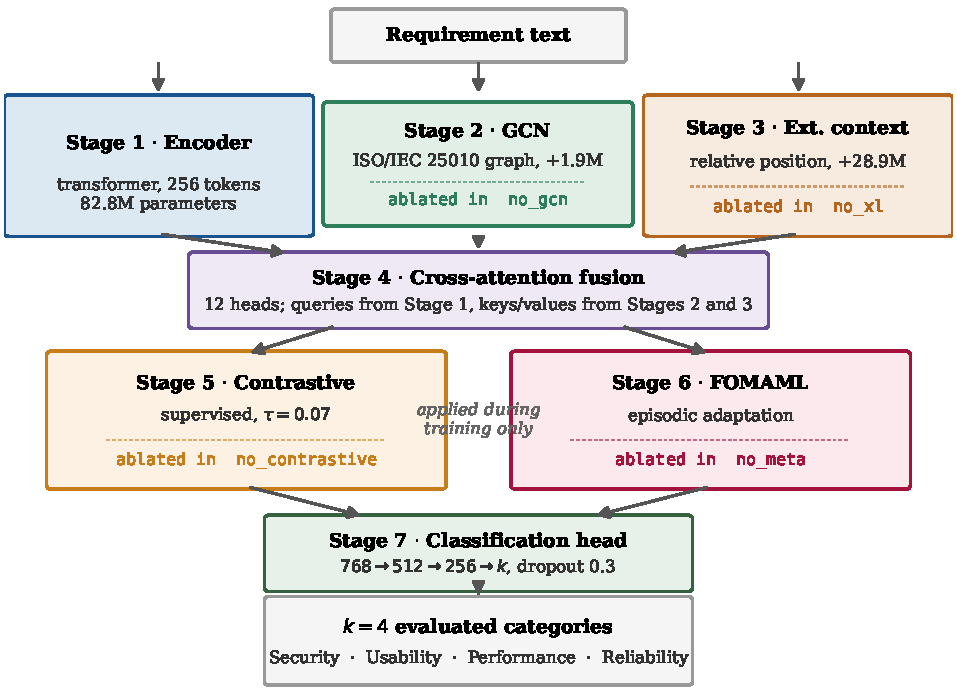
\includegraphics[width=\textwidth]{figures/fig_architecture.pdf}
\caption{The MAGNET-NFR architecture and its ablation points. Stages 1--3 build parallel
representations that Stage 4 fuses by cross-attention. Stages 5--6 shape the fused
representation during training only. The italic label in the corner of a box names the
variant in which that component is removed. Parameter counts are measured at run time rather than nominal. Removing the GCN reduces the model from 116.0M to 114.1M trainable
parameters, and removing the relative-position auxiliary block reduces it to 87.2M.}
\label{fig:architecture}
\end{figure}

Figure~\ref{fig:architecture} doubles as the map of the experiment. Each annotated
component corresponds to one ablation variant, and the parameter counts shown are those we
measured, confirming that each removal took effect rather than merely setting a flag. The
two objective-level ablations, contrastive loss and meta-learning, leave the
parameter count unchanged by construction.

\paragraph{Stage 1: contextual encoding.}
We encode each requirement with \texttt{distilroberta-base}, a six-layer distilled RoBERTa
variant with 82.8M parameters, capped at 256 tokens.

\paragraph{Stage 2: structured domain knowledge.}
A three-layer graph convolutional network operates over a knowledge graph specified as follows.
Nodes are terms: 40 ISO/IEC 25010 seed terms, ten per evaluated label, plus up to 200 mined
from the training split by TF-IDF over unigrams and bigrams with stop words removed and
$\mathrm{df} \geq 3$, giving 232 to 240 nodes per fold. Edges are
co-occurrence counts within a requirement, so $A_{ij}$ increments whenever terms $i$ and $j$
appear in the same training text. Node features are a learned embedding table of dimension $d = 768$ initialised randomly rather than from
pre-trained vectors.

How the graph signal becomes specific to the requirement being classified deserves explicit statement,
because it determines what the ablation tests. The graph is not pooled. The GCN produces an
$N \times d$ matrix of node representations that is identical for every requirement in a batch, and all
$N$ node vectors are passed to Stage 4 as individual key/value slots, concatenated with the
extended-context token states. The cross-attention query is the requirement's own \texttt{[CLS]}
representation, so while the node representations are input-invariant, the attention weights over them are
computed from each requirement separately and the graph contribution to the fused vector is therefore
requirement-conditioned.

This is a shared node bank read by requirement-specific attention, not requirement-specific subgraph
extraction, node masking or token-to-node matching. The distinction bounds the claim: our ablation tests
whether a globally shared, attention-addressed knowledge graph contributes, and a mechanism that selected
or reweighted nodes per requirement might behave differently. Node representations propagate as
\begin{equation}
H^{(l+1)} = \sigma\!\left(\tilde{D}^{-1} \tilde{A} H^{(l)} W^{(l)}\right),
\end{equation}
where $\tilde{A} = A + I$ is the adjacency matrix with self-loops added, $\tilde{D}$ is the
diagonal degree matrix of $\tilde{A}$, $H^{(l)}$ holds the node features at layer $l$,
$W^{(l)}$ is a learned weight matrix, and $\sigma$ is the rectified linear unit. We use the
row-stochastic normalisation $\tilde{D}^{-1}\tilde{A}$ rather than the symmetric
$\tilde{D}^{-1/2}\tilde{A}\tilde{D}^{-1/2}$ of Kipf and Welling~\cite{kipf2017}, which is
what our implementation computes. The two differ in how they weight high-degree nodes and
we did not compare them. The choice is recorded here so that the equation matches the
released code. The graph
is constructed from the training split of each fold only. Mining terms from the full corpus would leak test information into the graph.

\paragraph{Stage 3: extended context.}
Six transformer layers with a learned relative-position bias model dependencies across the
token sequence. This is a negative control rather than a test of long-context modelling. Median requirement
length is far below the 256-token window, so the mechanism has almost no opportunity to act
and its null result is expected rather than informative. We retain it because it was part of
the architecture as specified. This implements relative-position attention rather than the full
segment-recurrence mechanism of Dai et al.~\cite{dai2019}; with a median requirement
length well below the 256-token window, segment recurrence has no boundaries to cross on
this data.

\paragraph{Stage 4: cross-attention fusion.}
Multi-head cross-attention with 12 heads over $d = 768$ fuses the representations, taking the
encoder output as the query and the graph and extended-context representations concatenated
along the sequence axis as keys and values, with attention dropout 0.1. The output is added
residually to the encoder representation and layer-normalised. An ablated branch is removed
from the key/value concatenation rather than zeroed; when both are removed the fusion layer is
bypassed entirely, which is the encoder-only configuration.

\paragraph{Stage 5: supervised contrastive objective.}
A supervised contrastive term~\cite{khosla2020} with temperature $\tau = 0.07$ is added to
the cross-entropy loss:
\begin{equation}
\mathcal{L}_{\mathrm{con}}
= \frac{1}{|I|}\sum_{i \in I} \frac{-1}{|P(i)|}
\sum_{p \in P(i)} \log
\frac{\exp\!\left(\mathrm{sim}(z_i,z_p)/\tau\right)}
{\sum_{k \in A(i)}\exp\!\left(\mathrm{sim}(z_i,z_k)/\tau\right)} ,
\end{equation}
where $I$ indexes the anchors in a batch, $P(i)$ the positives sharing the label of anchor
$i$, $A(i)$ all other samples in the batch, $z$ the $\ell_2$-normalised projections, and
$\mathrm{sim}$ the dot product. Anchors with no positive contribute nothing, which under uniform sampling at batch size 16
falls unevenly. Auditing the released sampler, 100\% of Security anchors have a same-class
positive, against 75.5\% (Usability), 62.2\% (Performance) and 45.5\% (Reliability). The
objective therefore acts mainly on the majority class, making its ablation a weaker test of
what supervised contrastive learning could contribute under class-aware batching. A fully class-balanced sampler would introduce an oversampling confound, so we instead rerun the full and
no-contrastive configurations under an identical pair-aware sampler that guarantees every anchor a
same-class positive while preserving the empirical class mixture (Section~\ref{sec:protocolsens}).

\paragraph{Stage 6: first-order MAML.}
Episodic first-order model-agnostic meta-learning~\cite{finn2017} adapts the model on
sampled support sets and accumulates gradients from query-set loss. Because meta-learning results depend on how a task is defined, we state ours in full. A task is an $N$-way $K$-shot episode over the quality labels: $N = 3$ classes sampled
uniformly from the four evaluated labels, $K = 4$ support examples per class from the training
fold, and a disjoint query set of the same size. Eight episodes are drawn per epoch, one inner-loop step
at rate $10^{-3}$, and the first-order approximation omits the second-derivative term.

Two consequences follow. Episode classes are sampled uniformly rather than by frequency, so
the meta-objective sees a balanced task distribution the base objective does not; and tasks are
defined over labels rather than domains, so this tests few-shot adaptation across categories,
not the cross-domain adaptation that motivates meta-learning here. Testing that would need a
domain-partitioned split and project metadata the corpora lack.

\paragraph{Stage 7: classification head.}
A three-layer feed-forward network reduces the fused representation
$768 \rightarrow 512 \rightarrow 256 \rightarrow k$ with dropout 0.3, where $k = 4$.

\subsection{Experimental design}
\label{sec:design}

The design must satisfy two requirements that pull against each other. Isolating a component's contribution requires holding everything else constant, which is straightforward. Estimating per-category performance on categories holding 68 to 150 records requires evaluation support a conventional holdout cannot provide, which is not.

\paragraph{Cross-validation rather than a holdout.}
A conventional 70/15/15 split of this corpus leaves the minority categories with
single-digit test support, 16 Performance and 10 Reliability instances, from which a
per-category $F_1$ cannot be estimated with a usable confidence interval. We therefore use
stratified five-fold cross-validation repeated five times with independent fold
assignments. Each record receives exactly one out-of-fold prediction per repeat, from a
model that never saw it in training, and pooling folds yields prediction sets covering all
1{,}667 records. This increases minority-category evaluation support roughly sixfold at no cost in leakage, so that Reliability is evaluated on 68 predictions per repeat rather than 10.

\paragraph{Ablation protocol.}
Each variant removes exactly one component and is retrained from scratch. Folds, seeds,
hyperparameters, and class weighting are held constant, and no per-variant tuning was
performed. Within each fold, 15\% of the training partition is held out for model selection on macro $F_1$, and the held-out fold is never used for any selection decision. We verified
programmatically that no requirement identifier and no requirement text appears in both
the training and test portion of any fold, and that all pooled prediction sets cover an
identical item set.

\paragraph{Baselines.}
NoRBERT~\cite{hey2020} is re-trained on our folds using \texttt{bert-base-uncased}, which
makes the comparison internally fair but not directly comparable to the figure reported in
the original publication, since corpus and protocol differ. A TF-IDF pipeline with bigram
features and a class-weighted linear support vector machine provides a classical reference
on the same folds.

\paragraph{Hyperparameters.}
Table~\ref{tab:hyper} lists every setting. Two points about them matter for interpreting
the results. All configurations share identical values, so no variant is advantaged by
tuning. And the values are conventional defaults for transformer fine-tuning rather than the product of a search. We conducted no hyperparameter optimisation, for any
configuration, at any point. Section~\ref{sec:threats} treats the consequences of that
choice, which are the principal limitation of this study.

\begin{table}[htbp]
\centering
\caption{Hyperparameters, identical across all seven transformer configurations. No search was performed for the primary ablation; these are conventional defaults for transformer
fine-tuning. The equal-trial-budget tuning sensitivity of Section~\ref{sec:protocolsens} varies a subset of
them. Component
settings apply only to configurations retaining the component in question.}
\label{tab:hyper}
\small
\begin{tabular}{@{}llll@{}}
\toprule
\textbf{Scope} & \textbf{Setting} & \textbf{Value} & \textbf{Applies to}\\
\midrule
Optimisation & optimiser & AdamW & all\\
 & learning rate & $2 \times 10^{-5}$ & all\\
 & weight decay & 0.01 & all\\
 & batch size & 16 & all\\
 & epochs & 10 & all\\
 & gradient clipping & 1.0 & all\\
 & class weighting & balanced & all\\
 & model selection & best validation macro $F_1$ & all\\
\addlinespace
Encoding & backbone & \texttt{distilroberta-base} & MAGNET-NFR variants\\
 & maximum sequence length & 256 tokens & all\\
\addlinespace
Components & GCN layers & 3 & full, no\_xl, no\_con, no\_meta\\
 & extended-context layers & 6 & full, no\_gcn, no\_con, no\_meta\\
 & contrastive weight $\lambda$ & 0.1 & full, no\_gcn, no\_xl, no\_meta\\
 & contrastive temperature $\tau$ & 0.07 & full, no\_gcn, no\_xl, no\_meta\\
 & MAML episodes per epoch & 8 & full, no\_gcn, no\_xl, no\_con\\
 & MAML way / shot & 3 / 4 & full, no\_gcn, no\_xl, no\_con\\
 & MAML inner steps, inner rate & 1, $1 \times 10^{-3}$ & full, no\_gcn, no\_xl, no\_con\\
\addlinespace
Baselines & NoRBERT backbone & \texttt{bert-base-uncased} & NoRBERT\\
 & TF-IDF features & word 1--2 grams, min.\ df 2 & classical\\
 & SVM & linear, balanced class weights & classical\\
\bottomrule
\end{tabular}
\end{table}

\paragraph{Scale.}
Six MAGNET-NFR configurations and NoRBERT were each trained 25 times (five folds $\times$
five repeats), giving 175 transformer training runs and 25.1 GPU-hours on a single NVIDIA T4:
21.2 hours for the 150 MAGNET-NFR runs and 3.9 for the 25 NoRBERT runs. The classical
baseline, the matched-support experiment of Section~\ref{sec:support}, and the lexical
analysis together add under four minutes of CPU time, so total compute for the study is 25.1
hours to the nearest tenth.

\subsection{Statistical procedure}
\label{sec:stats}

Our claims concern macro $F_1$ on an imbalanced corpus, evaluated under repeated
cross-validation. Two properties of this setting determine the appropriate inference, and
both rule out the test most commonly used for paired classifier comparison.

McNemar's test compares error rates, not macro $F_1$. On a corpus where one category holds
80.6\% of records, accuracy and macro $F_1$ can move independently, so a test of the former
does not license a claim about the latter. Separately, repeated cross-validation produces
five correlated evaluations of the same 1{,}667 records. Pooling contingency counts across
repeats would treat 8{,}335 paired observations as independent when there are only 1{,}667
independent units, inflating the test statistic. In our data this inflation is material:
pooling gives $\chi^2 = 9.54$, $p = 0.002$ for the comparison between the full model and
the classical baseline, whereas no single repeat reaches significance (median
$p = 0.169$). We report this because the inflated figure is the one a conventional analysis
would produce.

We therefore use a \textbf{paired bootstrap over records} as the primary inferential
instrument. For each of 4{,}000 resamples we draw 1{,}667 records with replacement, compute
macro $F_1$ for both configurations on the resampled set in every repeat, average across
repeats, and record the difference. The resulting distribution yields a 95\% percentile
interval and a two-sided $p$-value. The statistic is the quantity our claims concern. We treat records as the resampling unit, which
is weaker than assuming independence: the corpus contains source clustering and near-duplicate
records, so the intervals give uncertainty conditional on the available out-of-fold predictions
under record-level resampling, not inference to a population of independently drawn
requirements.

\paragraph{Equivalence testing and the smallest effect of interest.}
A null result requires a stated threshold below which a difference is treated as
immaterial. We adopt a practical threshold of $\delta = 0.01$ macro $F_1$, and we are explicit that it
is interpretive rather than prespecified. It is an order of magnitude below the two to five
point gains routinely claimed for the components we ablate, and below the amplitude of the
late-epoch oscillation in validation macro $F_1$ that checkpoint selection alone introduces
(Section~\ref{sec:dynamics}), so a component contributing less than $\delta$ could not be
relied upon in practice even if it were real. Because a margin chosen after seeing the
estimates risks circularity, we report equivalence across four margins rather than resting on
one, and describe this as a retrospective equivalence sensitivity analysis rather than a
confirmatory test (Table~\ref{tab:equiv}).

The training objective combines cross-entropy with the contrastive term as
$L = L_{\mathrm{CE}} + \lambda L_{\mathrm{con}}$ with $\lambda = 0.1$, where
$L_{\mathrm{con}}$ operates on the output of a single linear projection head mapping the fused
representation from 768 to 256 dimensions followed by $\ell_2$ normalisation. In the
meta-learning configuration the inner loop adapts all trainable parameters, and the resulting
meta-gradient is summed with the ordinary classification gradient before the optimiser step
rather than applied in a separate pass.

We test equivalence by two one-sided tests at $\alpha = 0.05$, implemented as inclusion of
the 90\% bootstrap interval within $[-\delta, +\delta]$. We also report default JZS Bayes
factors~\cite{rouder2009} on the five per-repeat differences, which quantify evidence for
the null rather than merely failing to reject it. With five paired observations these
factors are weak by construction and we treat them as corroborative rather than primary.

We report the Friedman test across configurations on per-repeat macro $F_1$, the metric our
claims concern, as a descriptive check on rank stability, and Bonferroni correction at $\alpha' = 0.05/9 = 0.0056$. The family of nine comprises the full model against each of the four ablations, against
encoder-only, NoRBERT and the classical baseline, plus encoder-only and NoRBERT against the
classical baseline. Descriptive comparisons, such as the source holdouts, are not members. We did not conduct Shapiro--Wilk tests, Wilcoxon signed-rank tests across repeats, or
Cohen's $d$ on per-repeat means, and report none. With five repeats each has negligible
power. The two-sided Wilcoxon cannot return a $p$-value below 0.0625 at $n = 5$ regardless
of the data, and reporting these statistics alongside record-level intervals would invite
the reader to treat five correlated evaluations as five independent measurements. The
per-repeat means and standard deviations in Table~\ref{tab:results} convey the same
information without that implication.

\subsection{Reproducibility}
\label{sec:reproducibility}

We release the corpus with per-record provenance and source attribution, fold assignments,
both source spreadsheets, all code and prediction sets, and a verification script that
recomputes every quantitative claim and exits non-zero on any discrepancy. Rebuilding from
source reproduces the corpus and folds byte-for-byte.

% =====================================================================
\subsection{Robustness and methodological sensitivity protocols}
\label{sec:protocols}

The primary ablation is deliberately controlled at a fixed operating point. Five additional analyses,
reported in Sections~\ref{sec:loso} to \ref{sec:sixlabel}, address alternative explanations without
redefining that primary estimand. The last changes the task rather than the protocol, and is the only one
that alters the primary conclusion. Each protocol is specified here at the level a reader needs to judge
the design; runner scripts, frozen splits and per-fit outputs are in the replication package.

\paragraph{Neural leave-one-source-out.} For each source contributing at least 20 evaluated records, the
full composition, encoder-only and NoRBERT are trained on the remaining sources and tested on the held-out
collection, with a fixed training/validation partition. Single-class sources are reported as Security
recall. Of the four multi-class holdouts the three with at least 50 records form the descriptive mean; the
27-record collection is reported separately. No inferential interval is attached to that mean.

\paragraph{Limited equal-trial-budget nested tuning.} The full composition and encoder-only each receive
five candidate trials inside each of five outer folds. Selection uses only a fixed inner validation
partition; the outer fold is untouched until the selected configuration is retrained. The search spans
learning rate ($10^{-5}$ to $5\times10^{-5}$, log-uniform) and batch size (8, 16) for both, plus
contrastive weight (0.03--0.30) and MAML inner rate ($3\times10^{-4}$ to $3\times10^{-3}$) for the
composition. Trial 0 reproduces the primary defaults.

\paragraph{Near-duplicate-grouped cross-validation.} Character 3--5-gram TF-IDF cosine similarity
identifies pairs at or above 0.90; connected components form grouping units assigned wholly to one outer
fold, with group-safe inner validation. The full composition, encoder-only and the classical pipeline are
evaluated on the same grouped assignments.

\paragraph{Contrastive positive-pair audit and pair-aware sensitivity.} We estimate analytically, across
the 25 primary training splits, the probability that an anchor in a shuffled batch of 16 has at least one
same-label peer. The full and no-contrastive configurations are then rerun under an identical pair-aware
sampler in which each pair is drawn by class at empirical training frequency and contains two distinct
same-class examples. This guarantees positive eligibility without the oversampling confound a fully
balanced sampler would introduce.

\paragraph{Six-label task-definition sensitivity.} The corpus is rebuilt with the minimum class threshold
reduced from 40 to one, giving 1,719 requirements across six labels. Five repeated stratified five-fold
assignments are generated, every held-out fold contains all six labels, and the full composition and
encoder-only are retrained under the primary operating point, with the classical pipeline evaluated on the
same assignments. The $\pm 0.01$ margin and the 90\% interval criterion were frozen before the predictions
were analysed.

\paragraph{Six-label component ablation.} On the frozen six-label folds, four variants are retrained over
five repeats and five folds, giving 100 fits; the existing Full predictions are reused. Each contrast is
Full minus ablation with the same 4,000-resample paired record bootstrap. The four contrasts form one
multiplicity family: we control family-wise error on the tests by Holm adjustment and report
per-comparison 95\% estimation intervals, stating in Section~\ref{sec:sixcomp} where that distinction
affects a claim. The analysis is post-primary and exploratory; the freezing protocol is described there.

\paragraph{Matched-support resampling.} Each cap is evaluated over 40 subsamples drawn without
replacement. Under source stratification the target count is allocated in proportion to the capped
category's source shares, by integer floor allocation with remainder distribution and a random top-up for
any shortfall. The 40 draws cycle over the five original fold assignments.

\section{Results}
\label{sec:results}

We report the experiments in the order the research questions require. RQ1 and RQ2 concern whether the composed architecture improves on its parts, addressed first overall and then component by component. RQ3 concerns what accounts for the variation architecture does not, addressed through per-category results, a variance decomposition, and an experiment separating class support from category identity. A final subsection reports training dynamics.

\subsection{Overall performance}

The composed architecture performs well in absolute terms: 96.22\% $\pm$ 0.28 accuracy and
macro $F_1$ 0.8984 $\pm$ 0.0067, a margin of 15.66 points above the 80.56\% majority-class
floor, which on a four-class problem this imbalanced would ordinarily be reported as a
creditable result. The question is what produces it (Table~\ref{tab:results}).

\begin{table}[htbp]
\centering
\caption{Classification performance across six architectural configurations and two
baselines. Accuracy and macro $F_1$ are means over five repeats of stratified five-fold
cross-validation, pooled across all 1{,}667 records. $\Delta F_1$ and its interval come
from a paired bootstrap over records against the full model (4{,}000 resamples).
Bonferroni threshold for the nine comparisons drawn in this paper is
$\alpha' = 0.0056$.}
\label{tab:results}
\small
\setlength{\tabcolsep}{4pt}
\begin{tabular}{@{}lrrccrc@{}}
\toprule
\textbf{Configuration} & \textbf{Params} & \textbf{Min.} & \textbf{Accuracy (\%)} &
\textbf{Macro $F_1$} & \textbf{$\Delta F_1$ [95\% CI]} & \textbf{$p$}\\
\midrule
\multicolumn{7}{@{}l@{}}{\emph{Composed architecture and its ablations}}\\
Full MAGNET-NFR & 116.0M & 10.3 & 96.22 $\pm$ 0.28 & 0.8984 $\pm$ 0.0067 & n/a & n/a \\
$-$ GCN & 114.1M & 10.6 & 96.14 $\pm$ 1.08 & 0.8955 $\pm$ 0.0256 & $+$0.0029 [$-$0.0070, $+$0.0129] & 0.58\\
$-$ Relative-position block & 87.2M & 5.7 & 96.38 $\pm$ 0.23 & 0.8980 $\pm$ 0.0068 & $+$0.0005 [$-$0.0111, $+$0.0130] & 0.93\\
$-$ Contrastive loss & 116.0M & 10.7 & 96.09 $\pm$ 0.46 & 0.8933 $\pm$ 0.0140 & $+$0.0051 [$-$0.0045, $+$0.0145] & 0.29\\
$-$ Meta-learning & 116.0M & 8.9 & 96.30 $\pm$ 0.28 & 0.8983 $\pm$ 0.0054 & $+$0.0001 [$-$0.0089, $+$0.0092] & 1.00\\
Encoder only & 82.8M & 4.8 & 96.32 $\pm$ 0.40 & 0.8966 $\pm$ 0.0143 & $+$0.0018 [$-$0.0089, $+$0.0130] & 0.75\\
\midrule
\multicolumn{7}{@{}l@{}}{\emph{Baselines, identical folds}}\\
NoRBERT~\cite{hey2020} & 109.5M & 9.3 & 96.30 $\pm$ 0.23 & 0.8961 $\pm$ 0.0089 & $+$0.0023 [$-$0.0139, $+$0.0189] & 0.77\\
TF-IDF $+$ linear SVM & n/a & 0.1 & 95.48 $\pm$ 0.21 & 0.8730 $\pm$ 0.0065 & $+$0.0254 [$+$0.0011, $+$0.0496] & 0.042\\
\midrule
\emph{Majority-class floor} & n/a & n/a & \emph{80.56} & \emph{0.223} & n/a & n/a \\
\bottomrule
\end{tabular}
\setlength{\tabcolsep}{6pt}
\end{table}

Table~\ref{tab:results} is best read by column. The macro $F_1$ column spans 0.8933 to 0.8984
across seven transformer configurations, a range of 0.0051, smaller than the between-repeat
standard deviation of three of them: differences between architectures are smaller than
run-to-run variation within them. Every $\Delta F_1$ interval contains zero except the
classical baseline's, with half-widths between 0.009 and 0.016, and no ablation $p$-value falls
below 0.29. The parameter and time columns show the equivalence is not purchased at equal cost:
the encoder alone reaches within 0.0018 of the full model on 71\% of the parameters and 47\% of
the training time.

Two rows deserve separate comment. The $-$ GCN row has the widest accuracy standard
deviation, 1.08 against 0.23 to 0.46 elsewhere, which suggests that removing the graph
component destabilises training across folds without changing central performance. We tested this and cannot support it: Brown--Forsythe does not reject variance homogeneity
across the six configurations ($W = 0.65$, $p = 0.67$) or pairwise against the full model
($W = 0.87$, $p = 0.38$). At five observations the test has little power, so we record the
observation and decline the interpretation. The Encoder-only row is
the study's practical recommendation in a single line, being the cheapest transformer configuration and is statistically indistinguishable from the most expensive.

Even the classical baseline is close, and the evidence points two ways depending on what is
held fixed. Its deficit of 0.0254 is the largest in the table, but the record-level interval
reaches within 0.0011 of zero and $p = 0.042$ does not survive correction for the nine
comparisons drawn. Conditioning on this corpus and asking only whether the effect is consistent
across runs, the per-repeat differences give $\mathrm{BF}_{10} = 168$. The bootstrap asks
whether the advantage survives a fresh draw from the population; the per-repeat test asks only
whether training variance explains the gap. The advantage is robust to run-to-run variation but
only marginally to corpus variation, and we report the weaker reading.

Figure~\ref{fig:effects} presents every comparison as a difference with its interval.

\begin{figure}[htbp]
\centering
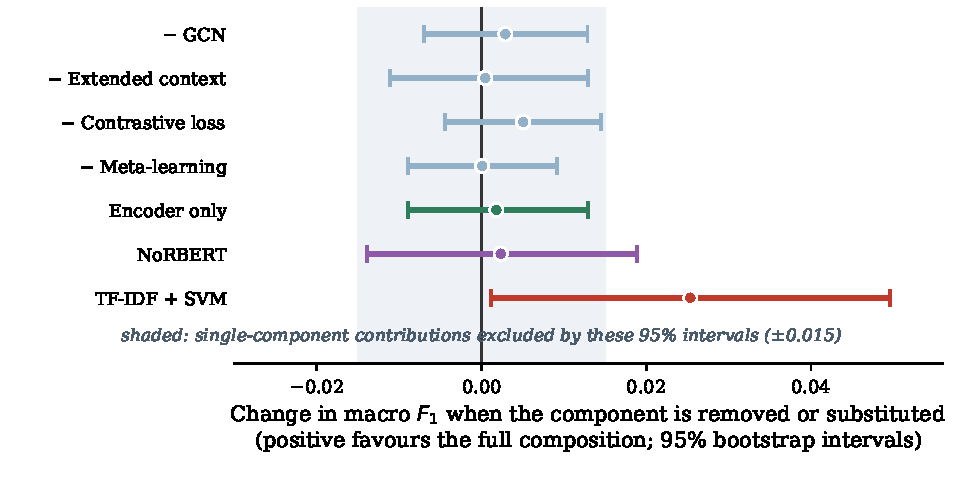
\includegraphics[width=\textwidth]{figures/fig_effects.pdf}
\caption{Change in macro $F_1$ from removing each component or substituting each baseline,
with 95\% intervals from a paired bootstrap over records. Positive values favour the full
composition. The shaded band marks single-component contributions the ablation intervals
exclude ($\pm$0.015). Every ablation interval spans zero; only the classical baseline
separates, and marginally. Numeric values and $p$-values are given in
Table~\ref{tab:results}.}
\label{fig:effects}
\end{figure}

Figure~\ref{fig:effects} shows the structure of the result directly. Six intervals
straddle zero, tightly. One clears it, barely. The figure's shape is the paper's argument:
whatever separates good from poor performance on this task, it is not the presence or
absence of these architectural components.

\subsection{No component contributes measurably}
\label{sec:ablation}

The five ablations change macro $F_1$ by between 0.0001 and 0.0051, and every interval
contains zero ($0.29 \leq p \leq 1.00$). A Friedman test across all seven transformer configurations, computed on per-repeat macro
$F_1$ so that it uses the metric carrying our claims rather than accuracy, does not reject
equality of average ranks ($\chi^2 = 2.49$, df $= 6$, $p = 0.87$), with mean ranks spanning
3.2 to 4.8 where seven tied configurations would each rank 4.0. We report this for completeness rather than as evidence of equivalence, since with five blocks and seven treatments the test has little power, so its failure to reject carries
limited information. The interval estimates carry the equivalence claim.

A null result is informative only insofar as the design could have detected an effect, so we
state what the intervals exclude rather than resting on non-significance. Two inferential statements are involved and we keep them apart. The 95\% estimation intervals
of Table~\ref{tab:results} bound each effect: the worst upper bound among the four
single-component ablations is 0.0145, so effects above roughly 0.015 lie outside every 95\%
interval. The 90\% intervals of Table~\ref{tab:equiv} serve the two one-sided tests, a stricter
question, and establish equivalence at $\delta = 0.015$ for all four but at $\delta = 0.010$
only for meta-learning.

\begin{table}[htbp]
\centering
\caption{Equivalence testing across four candidate margins. Equivalence requires the 90\%
bootstrap interval to lie entirely within $[-\delta, +\delta]$, the interval-inclusion form of
two one-sided tests at $\alpha = 0.05$. We report a range of margins rather than a single
value because our practical threshold of 0.01 is interpretive rather than prespecified
(Section~\ref{sec:stats}). Bayes factors are default JZS factors on the five per-repeat
differences; $\mathrm{BF}_{01} > 3$ would constitute moderate evidence for the null.}
\label{tab:equiv}
\small
\setlength{\tabcolsep}{5pt}
\begin{tabular}{@{}lrccccc r@{}}
\toprule
& & & \multicolumn{4}{c}{\textbf{Equivalent at $\delta =$}} & \\
\cmidrule(lr){4-7}
\textbf{Comparison} & \textbf{$\Delta F_1$} & \textbf{90\% interval} & \textbf{.005} & \textbf{.010} & \textbf{.015} & \textbf{.020} & \textbf{$\mathrm{BF}_{01}$}\\
\midrule
$-$ GCN & $+$0.0029 & [$-$0.0054, $+$0.0113] & no & no & yes & yes & 2.4\\
$-$ Relative-position block & $+$0.0005 & [$-$0.0092, $+$0.0110] & no & no & yes & yes & 2.5\\
$-$ Contrastive loss & $+$0.0051 & [$-$0.0029, $+$0.0129] & no & no & yes & yes & 1.8\\
$-$ Meta-learning & $+$0.0001 & [$-$0.0075, $+$0.0079] & no & \textbf{yes} & yes & yes & 2.5\\
Encoder only & $+$0.0018 & [$-$0.0073, $+$0.0111] & no & no & yes & yes & 2.4\\
\midrule
NoRBERT & $+$0.0023 & [$-$0.0114, $+$0.0165] & no & no & no & yes & 2.1\\
TF-IDF $+$ linear SVM & $+$0.0254 & [$+$0.0053, $+$0.0460] & no & no & no & no & 0.006\\
\bottomrule
\end{tabular}
\setlength{\tabcolsep}{6pt}
\end{table}

Table~\ref{tab:equiv} obliges us to state the result narrowly, and the margin matters. At
$\delta = 0.01$ only the meta-learning ablation is formally equivalent; the other three and the
encoder-only comparison have 90\% intervals extending just past the threshold. At
$\delta = 0.015$ all four single-component ablations and the encoder-only comparison are
equivalent, and at $\delta = 0.005$ none is. The defensible statement is therefore that no
95\% estimation interval admits a single-component effect above 0.015, that equivalence is
established at margins of 0.015 and wider, and that it cannot be established at 0.010 or
0.005. The band below 0.015 is resolution this corpus does not have.

The Bayes factors say the same in a different currency. Across the five ablation comparisons
$\mathrm{BF}_{01}$ ranges from 1.8 to 2.5, evidence favouring the null but short of the
conventional threshold of 3 for moderate evidence. We therefore describe the components as
making no contribution the design can resolve, rather than as making no contribution, and we
do not claim demonstrated equivalence at the conventional bound.

Detection depends on interval width as well as effect size, and the two do not order together
here. The classical deficit is resolved against the full model ($+0.0254$, $p = 0.042$) and
NoRBERT ($+0.0230$, $p = 0.041$) but not against the encoder alone ($+0.0236$, $p = 0.057$),
which carries a wider interval. The design resolves differences near 0.024 inconsistently and excludes those above 0.015 reliably; the
intervening band is beyond what this corpus settles. All five ablations fall well below that band.

Removing the GCN, the component the architecture's rationale weights most heavily,
changes macro $F_1$ by 0.0029 with an interval of $[-0.0070, +0.0129]$. Removing
meta-learning changes it by 0.0001. Removing the relative-position auxiliary block changes it by
0.0005 while eliminating 28.9M parameters and 45\% of training time, indicating that the
component consumed resources without contributing discriminative capacity.

The most direct test is the encoder-only configuration, which removes all four additional
paradigms simultaneously. It differs from the full composition by 0.0018 macro $F_1$ ($p = 0.75$), less than the difference produced by removing the contrastive objective alone, and in the same direction. Whatever the four components contribute individually,
their combined contribution is not distinguishable from zero.

\subsection{Cross-architecture corroboration}
\label{sec:norbert}

NoRBERT provides a cross-architecture check rather than an independent replication: we executed
it ourselves, on the same corpus and folds. What it offers is corroboration from an architecture
we did not design. Trained on identical folds it
attains macro $F_1$ 0.8961 $\pm$ 0.0089, differing from the full composition by 0.0023
($p = 0.77$) and from our encoder-only configuration by 0.0005. It uses a different
pre-trained encoder (\texttt{bert-base-uncased} rather than
\texttt{distilroberta-base}), a different training procedure, and was developed
independently. Three transformer approaches converge within 0.0023 macro $F_1$, which is consistent with a possible data
or annotation ceiling, and equally consistent with shared pre-training, a shared optimisation recipe or a
common representational limit. Without a human baseline we cannot distinguish these, and the six-label
result of Section~\ref{sec:sixlabel} weighs against the strongest reading, since the same architectures
separate once the label space changes.

\subsection{Generalisation to an unseen source}
\label{sec:loso}

Record-level cross-validation allows requirements from the same collection to appear in training and
test folds, so source-specific wording may inflate absolute performance. Because one collection supplies
64.2\% of records, this matters here. We therefore evaluate Full MAGNET-NFR, encoder-only and NoRBERT
under leave-one-source-out, training on all collections but one and testing on the held-out collection,
retaining the classical pipeline as a reference. Table~\ref{tab:loso} keeps the metric distinction
explicit: four held-out collections contain multiple evaluated labels and use macro $F_1$; two are
Security-only and use recall.

\begin{table}[htbp]
\centering
\caption{Leave-one-source-out evaluation. Values are macro $F_1$ for multi-class sources and Security
recall for single-class sources. The primary descriptive mean is over the three multi-class holdouts with
at least 50 records. The 27-record CPN holdout is reported separately because all three neural
configurations collapsed to a single predicted label on it, returning identical macro $F_1$; it is a
diagnostic of failure under extreme source shift rather than a performance estimate.}
\label{tab:loso}
\small
\setlength{\tabcolsep}{5pt}
\begin{tabular}{@{}lrrrrrr@{}}
\toprule
\textbf{Held-out collection} & \textbf{n} & \textbf{Classes} & \textbf{Full} & \textbf{Encoder} & \textbf{NoRBERT} & \textbf{TF-IDF}\\
\midrule
\multicolumn{7}{@{}l@{}}{\emph{Multi-class holdouts: macro $F_1$}}\\
Curated Mendeley collection & 57 & 4 & 0.808 & 0.856 & 0.856 & 0.636\\
promise\_exp & 165 & 4 & 0.801 & 0.802 & 0.741 & 0.699\\
software\_requirements\_extended & 237 & 4 & 0.754 & 0.773 & 0.736 & 0.688\\
\quad \textbf{mean, multi-class $n \geq 50$} & & & \textbf{0.788} & \textbf{0.810} & \textbf{0.778} & \textbf{0.674}\\
\addlinespace
\multicolumn{7}{@{}l@{}}{\emph{Collapse diagnostic}}\\
SecReq Customer Premises Network & 27 & 3 & 0.180 & 0.180 & 0.180 & 0.407\\
\addlinespace
\multicolumn{7}{@{}l@{}}{\emph{Single-class holdouts: Security recall}}\\
PURE\_and\_others & 1{,}071 & 1 & 0.868 & 0.852 & 0.866 & 0.864\\
requirements\_MoSCoW & 108 & 1 & 0.935 & 0.926 & 0.898 & 0.991\\
\bottomrule
\end{tabular}
\setlength{\tabcolsep}{6pt}
\end{table}

The neural results close the architectural source-shift objection rather than merely showing that source
shift exists. Across the three multi-class holdouts with at least 50 records, the full composition
averages 0.788 macro $F_1$, below encoder-only at 0.810 and above NoRBERT at 0.778, with TF-IDF at 0.674.
Full is lower than encoder-only on each of these three holdouts. Source shift is substantial, but it does
not reveal a benefit from composition.

The 27-record CPN holdout behaves differently and is excluded from the primary mean for a specific
reason. All three neural configurations returned macro $F_1 = 0.180180$, identical to six decimal places,
which is exactly the value obtained by predicting Security for all 27 records against its composition of
15 Performance, 10 Security and 2 Usability. The neural models did not produce noisy estimates here; they
collapsed to a single label. TF-IDF scored 0.407 and retained some discrimination. Under the most severe
source shift the corpus affords, the classical pipeline degraded while every neural configuration failed
outright. The holdout is too small to carry weight alone, but the contrast is consistent with the rest of
the paper: composition did not confer robustness where robustness was most needed.

Because source and label remain confounded and some holdouts are small, these results are sensitivity
evidence rather than a clean estimate of deployment performance. The single-class holdouts cannot answer
the four-way discrimination question and their recall values are reported only as source-specific
diagnostics.

\subsection{Protocol sensitivities}
\label{sec:protocolsens}

Three further analyses ask whether a protocol artefact explains the four-label null rather than the
absence of an architectural effect. Each is specified in Section~\ref{sec:protocols}; each contrasts the
full composition against a comparator under a changed protocol while holding the estimand fixed.
Table~\ref{tab:sens} reports all three.

\begin{table}[htbp]
\centering
\caption{Protocol sensitivities on the four-label task. Each row changes one aspect of the evaluation and
re-estimates the contrast with the same 4,000-resample paired record bootstrap. ``Equiv.\ $\pm 0.01$''
asks whether the 90\% interval lies inside the interpretive margin. None of the three establishes an
aggregate advantage for the composition.}
\label{tab:sens}
\small
\setlength{\tabcolsep}{4pt}
\begin{tabular}{@{}llrrrc@{}}
\toprule
\textbf{Sensitivity} & \textbf{Contrast} & \textbf{Full} & \textbf{Comp.} & \textbf{$\Delta F_1$ [95\% CI]} & \textbf{Equiv.}\\
\midrule
Equal-trial-budget tuning & Full $-$ Encoder & 0.9010 & 0.8923 & $+$0.0087 [$-$0.0152, $+$0.0337] & no\\
Near-duplicate-grouped CV & Full $-$ Encoder & 0.8754 & 0.8816 & $-$0.0063 [$-$0.0171, $+$0.0042] & no\\
Pair-aware contrastive & Full $-$ No-con. & 0.8869 & 0.8872 & $-$0.0003 [$-$0.0090, $+$0.0087] & \textbf{yes}\\
\bottomrule
\end{tabular}
\setlength{\tabcolsep}{6pt}
\end{table}

Each row answers a distinct objection, and the three differ in evidential strength.

Equal-trial-budget tuning addresses the possibility that fixed defaults disadvantage a more
hyperparameter-sensitive composition. Both architectures received 25 inner trials with outer test folds
untouched. The point estimate favours the composition but the interval admits both a meaningful advantage
and a meaningful disadvantage, so it establishes neither benefit nor equivalence. Equal trial counts are
also not equal search adequacy: encoder-only searches two dimensions and the composition four, so five
trials cover the larger space more thinly. That asymmetry runs against the null rather than toward it. What
the experiment shows is only that a small equal-trial budget does not reverse the primary result.

Near-duplicate-grouped cross-validation removes template leakage. Under the original random folds,
75.4--89.0\% of the 118 detected near-duplicate pairs cross train/test boundaries; grouped splitting
reduces this to zero in every repeat. Absolute macro $F_1$ falls for every method, by approximately 0.023
for Full, 0.015 for encoder-only and 0.032 for the classical pipeline, confirming that template similarity
inflated the original absolute scores. The architectural conclusion survives, with encoder-only holding the
higher grouped mean, though the interval extends past $-0.01$ so this is not strict equivalence.
Repeating the CPU-only cluster construction at cosine thresholds of 0.85 and 0.95 leaves the grouped
classical macro $F_1$ below its record-random value of 0.8730 at all three thresholds (0.8277, 0.8409 and
0.8215 respectively), so the direction of the leakage correction is not an artefact of the cutoff. No
neural fits were run at the neighbouring thresholds, so the neural comparison remains conditional on the
0.90 rule. Cluster counts and the full sensitivity are in the replication package.

Pair-aware contrastive batching is the strongest of the three. The batch audit found that under ordinary
shuffling only 46.0\% of Reliability anchor exposures have a same-class positive, against 62.2\% for
Performance, 75.5\% for Usability and effectively 100\% for Security, so the objective is applied far less
often to the smallest class. Rerunning the full and no-contrastive configurations under an identical
pair-aware sampler leaves them within 0.0003 macro $F_1$, with the complete 95\% interval inside the
$\pm 0.01$ margin. This is the only new analysis to establish practical equivalence, and it is
sampler-specific: it does not replace the ordinary-batch primary estimate of $+0.0051$
[$-$0.0045, $+$0.0145], and it is not a claim that the contrastive objective is inert under arbitrary
batching.

\subsection{Six-label task-definition sensitivity}
\label{sec:sixlabel}

Every result above rests on a task from which two mapped labels were removed. Maintainability (34 records)
and Portability (18) fall below the 40-record precision rule of Section~\ref{sec:corpus}, and excluding
them is defensible for class-specific precision but changes the learning problem. Because the components
under test are often motivated by low-resource performance, this is the scope decision most likely to
matter. We therefore rebuild the corpus with the threshold lowered to one, giving 1,719 records across all
six labels with a majority-class floor of 78.13\%, generate five repeated stratified five-fold assignments
in which every held-out fold contains all six labels, and retrain the full composition and encoder-only
under the primary operating point. This is 50 further fits, reported in Table~\ref{tab:sixlabel}. The $\pm 0.01$ margin and the 90\%
interval criterion were frozen before the predictions were examined.

\begin{table}[htbp]
\centering
\caption{Six-label sensitivity over five repeated stratified five-fold prediction sets. Accuracy and macro
$F_1$ are mean $\pm$ SD across repeats. The paired contrast is Full minus encoder-only over 4,000
record-level bootstrap resamples, conditional on the fixed six-label corpus.}
\label{tab:sixlabel}
\small
\begin{tabular}{@{}lrr@{}}
\toprule
\textbf{Configuration} & \textbf{Accuracy} & \textbf{Macro $F_1$}\\
\midrule
Full MAGNET-NFR & 0.9499 $\pm$ 0.0025 & 0.8286 $\pm$ 0.0113\\
Encoder-only & 0.9425 $\pm$ 0.0034 & 0.8038 $\pm$ 0.0088\\
TF-IDF $+$ linear SVM & 0.9393 $\pm$ 0.0031 & 0.7681 $\pm$ 0.0231\\
\bottomrule
\end{tabular}

\smallskip
{\small Full $-$ Encoder: $\Delta F_1 = +0.0248$; 95\% CI $[+0.0044, +0.0469]$; 90\% CI
$[+0.0079, +0.0437]$, not contained in $\pm 0.01$; $p = 0.016$.}
\end{table}

The six-label task does not reproduce the near-null primary comparison. Conditional on this corpus, the
interval lies above zero and the 90\% interval is not inside the equivalence margin. The broader task is
also harder for every method: the classical pipeline falls from 0.8730 macro $F_1$ on four labels to
0.7681 on six.

\begin{table}[htbp]
\centering
\caption{Class-wise mean $F_1$ across the five six-label repeat-pooled prediction sets, with each label's
contribution to the aggregate macro-$F_1$ difference. Differences are Full minus encoder-only and are
descriptive; no class-specific inferential claim is made.}
\label{tab:sixclasswise}
\small
\begin{tabular}{@{}lrrrrr@{}}
\toprule
\textbf{Label} & \textbf{n} & \textbf{Full} & \textbf{Encoder-only} & \textbf{$\Delta F_1$} & \textbf{Share of macro $\Delta$}\\
\midrule
Security & 1{,}343 & 0.9803 & 0.9771 & $+$0.0032 & 2.2\%\\
Usability & 150 & 0.8743 & 0.8495 & $+$0.0248 & 16.7\%\\
Performance & 106 & 0.8929 & 0.8750 & $+$0.0179 & 12.0\%\\
Reliability & 68 & 0.7776 & 0.7626 & $+$0.0151 & 10.1\%\\
Maintainability & 34 & 0.6411 & 0.5773 & $+$0.0638 & 42.9\%\\
Portability & 18 & 0.8052 & 0.7813 & $+$0.0239 & 16.1\%\\
\bottomrule
\end{tabular}
\end{table}

Two features of Table~\ref{tab:sixclasswise} bear on how the result should be read, and they pull in
opposite directions.

The advantage is not confined to the restored labels. Maintainability and Portability together contribute
59\% of the aggregate difference from 3.0\% of the records, but the remaining 41\% comes from the four
labels that also appear in the primary task. Evaluating the six-label models on those four labels alone
gives Full 0.8813 against encoder-only 0.8660, a gap of $+0.0152$, where the primary four-label experiment
gave $+0.0018$. The same labels and the same records yield an eight-fold larger gap when the models were
trained on six classes. What changed is the training problem, not merely the set of categories being
scored, so the six-label result is not simply a matter of the composition classifying rare labels better.

Against that, the single largest contributor is very thin. Maintainability supplies 42.9\% of the
aggregate difference from 34 records, and its mean gap of 0.0638 corresponds to 2.8 additional correct
predictions per repeat, 19.8 against 17.0. Its sign reverses in one of the five repeats and its per-repeat
difference ranges from $-0.008$ to $+0.142$. Portability behaves similarly at $n = 18$, where Full leads by
one or two records in three repeats and is level in two. The aggregate interval is computed over records
and is not invalidated by this, but a reader should know that a substantial share of the headline
difference turns on a handful of predictions in the two smallest classes.

The appropriate reading is therefore that label-space definition moderates the architectural comparison on
this corpus. It is not evidence that the composition is generally superior on six-label NFR classification,
because the restored labels are very small and the source concentration and annotation limits of
Section~\ref{sec:corpus} are unchanged. Section~\ref{sec:sixcomp} takes up which component produces the advantage.

\subsection{Six-label component-ablation follow-up}
\label{sec:sixcomp}

The endpoint comparison of Section~\ref{sec:sixlabel} shows that the architectural conclusion changes with
the label space but cannot say which mechanism is responsible, because only the two endpoints were
retrained. We therefore ran a component ablation on the same frozen six-label task.

This analysis is post-primary. It was initiated after the endpoint difference had been observed, so it is
exploratory with respect to the original hypothesis family and we report it as such throughout. Before the
four new prediction sets were examined we froze the corpus, the five repeated stratified five-fold
assignments, the operating point, the existing Full predictions, the four ablations, the contrast
definition, the bootstrap procedure, the multiplicity family and the $\pm 0.01$ equivalence rule. Four
variants were retrained over five repeats and five folds, giving 25 fits each and 100 new fits; Full was
not retrained. Table~\ref{tab:sixcomp} reports the outcome. Each contrast is Full minus ablation on repeat-pooled macro $F_1$, with 4,000 paired
record-level bootstrap resamples and sampled item positions carried across all repeats and both models.

\begin{table}[htbp]
\centering
\caption{Six-label component ablation against the frozen Full predictions. Contrasts are Full minus
ablation, so a positive value means removing the component costs performance. Ordinary 95\% intervals
describe estimation; the Bonferroni 98.75\% intervals and Holm-adjusted bootstrap $p$-values address the
four-comparison family. Equivalence requires the 90\% interval to lie within $\pm 0.01$.}
\label{tab:sixcomp}
\small
\setlength{\tabcolsep}{4pt}
\begin{tabular}{@{}lrrllrc@{}}
\toprule
\textbf{Removed} & \textbf{Full} & \textbf{Abl.} & \textbf{95\% CI} & \textbf{Bonf.\ 98.75\% CI} & \textbf{Holm $p$} & \textbf{Equiv.}\\
\midrule
GCN & 0.8286 & 0.8061 & [$+$0.0070, $+$0.0404] & [$+$0.0023, $+$0.0474] & 0.0165 & no\\
Contrastive objective & 0.8286 & 0.8078 & [$+$0.0090, $+$0.0332] & [$+$0.0054, $+$0.0371] & 0.0040 & no\\
Meta-learning & 0.8286 & 0.8141 & [$-$0.0039, $+$0.0342] & [$-$0.0097, $+$0.0407] & 0.2269 & no\\
Relative-position block & 0.8286 & 0.8191 & [$-$0.0082, $+$0.0280] & [$-$0.0143, $+$0.0334] & 0.3139 & no\\
\midrule
\multicolumn{3}{@{}l}{\emph{Sum of the four marginal effects}} & \multicolumn{4}{l}{\emph{$+$0.0671}}\\
\multicolumn{3}{@{}l}{\emph{Full $-$ Encoder (all four removed)}} & \multicolumn{4}{l}{\emph{$+$0.0248, 95\% CI [$+$0.0044, $+$0.0469]}}\\
\bottomrule
\end{tabular}
\setlength{\tabcolsep}{6pt}
\end{table}

Two contrasts resolve. Removing the GCN costs 0.0225 macro $F_1$ and removing the contrastive objective
costs 0.0207, and for both the Bonferroni 98.75\% interval remains above zero, so the result does not
depend on reading per-comparison intervals as if they were family-wise. Removing meta-learning or the
relative-position block leaves both the 95\% and the family-wise intervals spanning zero. No contrast
satisfies the frozen equivalence criterion, so the two unresolved components are unresolved rather than
shown to be inert.

The marginal effects are strongly non-additive, and the arithmetic is worth stating plainly. The four sum
to $+0.0671$, while removing all four simultaneously, which is the Full-versus-encoder contrast, costs only
$+0.0248$. The sum is 2.7 times the joint effect. Each component therefore recovers performance that the
others partly supply in its absence, so these are marginal removal effects at the full configuration and
not a decomposition of the endpoint difference. Attributing $+0.0225$ of the $+0.0248$ gap to the GCN would
be a misreading of what a one-at-a-time ablation measures.

The result sits in tension with the primary experiment, and we state the tension rather than resolve it.
The same GCN ablation changes macro $F_1$ by $+0.0029$ on four labels, with an interval spanning zero, and
by $+0.0225$ on six. The same corpus, architecture and operating point yield an eight-fold difference in
the measured effect of one component after adding 52 records in two classes. Three readings are available
and the design does not separate them. The components may contribute specifically where labelled data is
scarcest, which is where they are usually motivated. The six-label task may simply be harder, so the same
mechanism yields a larger measurable effect further from ceiling. Or the four-label experiment may have had
too little resolution to detect an effect of this size, since its design excludes single-component effects
above roughly 0.015 and $+0.0225$ sits just beyond that bound. Distinguishing these requires label spaces
intermediate between four and six, or an independent corpus with adequate minority-class support.

The class-wise pattern is suggestive and we report it as a diagnostic only. GCN removal loses most on
Maintainability ($+0.0532$) and Reliability ($+0.0331$); contrastive removal on Portability ($+0.0449$),
Maintainability ($+0.0313$) and Reliability ($+0.0280$); and meta-learning removal shows a large Portability
contrast ($+0.0531$) despite an aggregate effect that does not resolve. Both resolving components therefore
lose most where labelled data is scarcest, which is where they are usually motivated. Rare-label support
and the absence of a class-wise multiplicity family preclude confirmatory class-specific claims, so this
pattern motivates the mechanism question rather than answering it.

A reader should weigh what the follow-up does not establish. It is exploratory and post-primary, and the
two restored labels hold 34 and 18 records, so the class-wise diagnostics above rest on very few
predictions.

\subsection{Category, not architecture, governs performance}
\label{sec:support}

Sections~\ref{sec:ablation} and \ref{sec:norbert} establish that method choice moves macro
$F_1$ very little on this corpus. Something moves it a great deal, and this section identifies
what. The per-category results for the full model and the two principal baselines appear in
Table~\ref{tab:percat}.

\begin{table}[htbp]
\centering
\caption{Per-category performance, averaged over five repeats of pooled out-of-fold
prediction. Precision and recall are reported for the full model; the $F_1$ columns permit
comparison across configurations.}
\label{tab:percat}
\small
\begin{tabular}{@{}lrccccc@{}}
\toprule
& & \multicolumn{3}{c}{\textbf{Full MAGNET-NFR}} & \textbf{NoRBERT} & \textbf{TF-IDF + SVM}\\
\cmidrule(lr){3-5}\cmidrule(lr){6-6}\cmidrule(lr){7-7}
\textbf{Category} & \textbf{Support} & \textbf{Precision} & \textbf{Recall} & \textbf{$F_1$} & \textbf{$F_1$} & \textbf{$F_1$}\\
\midrule
Security    & 1{,}343 & 0.980 & 0.984 & 0.982 $\pm$ 0.002 & 0.983 $\pm$ 0.001 & 0.980\\
Usability   & 150 & 0.901 & 0.873 & 0.887 $\pm$ 0.004 & 0.889 $\pm$ 0.004 & 0.876\\
Performance & 106 & 0.893 & 0.938 & 0.914 $\pm$ 0.017 & 0.904 $\pm$ 0.019 & 0.879\\
Reliability & 68 & 0.858 & 0.771 & 0.811 $\pm$ 0.012 & 0.808 $\pm$ 0.032 & 0.786\\
\midrule
\textbf{Macro average} & 1{,}667 & 0.908 & 0.892 & \textbf{0.898 $\pm$ 0.007} & 0.896 $\pm$ 0.009 & 0.873\\
\bottomrule
\end{tabular}
\end{table}

Table~\ref{tab:percat} exposes the strongest regularity in our results. Per-category performance declines
with support from 0.982 for Security to 0.811 for Reliability, a range of 0.171, roughly seven times the
largest difference between any two methods, and the ordering is identical across all three methods, which
differ by at most 0.035 within any row. The decline is driven by recall, Reliability precision being 0.858
against recall 0.771, so the classifier is conservative rather than confused. Standard deviations widen
monotonically as support falls, from $\pm$0.002 to $\pm$0.012, so categories with less labelled data are
classified both worse and less consistently. Kurtanović and Maalej~\cite{kurtanovic2017} likewise report
their highest precision and recall for security and performance.

Figure~\ref{fig:support} quantifies the comparison between category and method effects,
and then isolates the role of support.

\begin{figure}[htbp]
\centering
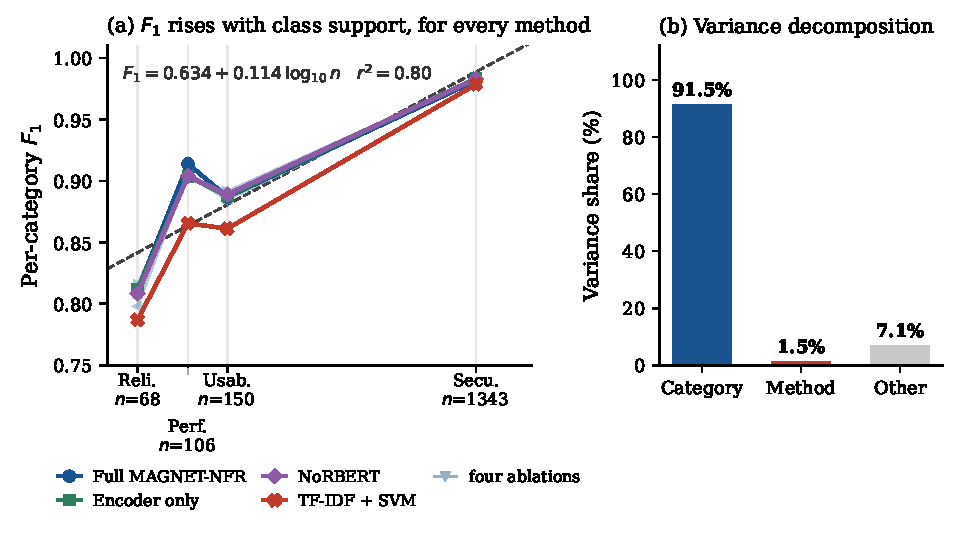
\includegraphics[width=\textwidth]{figures/fig_support.pdf}
\caption{Category accounts for more of the observed variation than architectural choice.
(a) Per-category $F_1$ against class support for all eight methods, with the four ablation
variants in light grey and a least-squares fit over method--category means; the fit rests on
four distinct support values, so it is descriptive rather than independent evidence of a
support--performance relationship. (b) Descriptive decomposition of the variance in per-category $F_1$. The third bar aggregates the repeat
main effect (1.6\%), the category-by-method interaction (0.7\%) and the residual (4.8\%); it is not
residual alone. The matched-support experiment appears separately in Figure~\ref{fig:matched}.}
\label{fig:support}
\end{figure}

Figure~\ref{fig:support}(a) shows the eight methods tracing a common curve, fitted over
method--category means as $F_1 = 0.634 + 0.114\log_{10} n$ with $r^2 = 0.80$.
Figure~\ref{fig:support}(b) partitions the variance in per-category $F_1$ over the 160 cells
formed by eight methods, four categories and five repeats. We compute type-I sums of squares for category, method and repeat as main effects plus a
category-by-method interaction, each as a share of the total about the grand mean. Cells are
equally sized, so unequal category support enters through the $F_1$ values rather than the
weighting. Under this descriptive partition category accounts for 91.5\% of the observed variation, method
for 1.5\%, repeat for 1.6\%, the interaction for 0.7\% and the residual for 4.8\%. We report this as a descriptive partition and attach no interval to the shares. A bootstrap over the 160
cells would misstate the uncertainty, because the cells are not independent: every method predicts the same
records and every repeat reuses the same corpus, so resampling cells destroys the factorial dependence the
design creates. An interval aligned with the data-generating unit would resample records, carry every
method and repeat prediction for each sampled record, and redo the decomposition inside each resample. We
have not done this, and therefore treat the 91.5\% against 1.5\% contrast as descriptive evidence of
separation rather than as an estimated quantity with known precision.

These are associational results, and category identity confounds class support with
whatever else distinguishes one quality attribute from another. We therefore ran a
matched-support experiment to separate the two components. Capping Security's
\emph{training} support at successively lower levels while leaving the evaluation set
untouched isolates the contribution of labelled-data volume from that of category
identity. Table~\ref{tab:matched} reports the result.

\begin{table}[htbp]
\centering
\caption{Matched-support experiment, run with the TF-IDF and linear SVM pipeline so that 40 subsamples
per level are affordable; the effect sizes here are therefore not directly comparable with the
transformer ablation contrasts in Table~\ref{tab:results}. The capped category's training pool is reduced
to each level while its evaluation set is held fixed. Levels are the size of the available category
pool before fold partitioning; the mean number of records actually seen by a fitted model is
smaller by the fold and validation split, and is given in the final column for the native
level. Each cell is the mean over 40 independent subsamples drawn to preserve the source
composition of the capped category, with the 95\% range across subsamples in brackets.}
\label{tab:matched}
\small
\setlength{\tabcolsep}{5pt}
\begin{tabular}{@{}lrrl r@{}}
\toprule
\textbf{Capped category} & \textbf{Pool before folds} & \textbf{$F_1$} & \textbf{95\% range} & \textbf{Train/fold}\\
\midrule
Security & 1{,}343 & 0.979 & [0.978, 0.980] & 913\\
         &    600 & 0.978 & [0.976, 0.981] & \\
         &    300 & 0.973 & [0.969, 0.976] & \\
         &    150 & 0.955 & [0.950, 0.959] & \\
         &    106 & 0.936 & [0.930, 0.943] & \\
         &     68 & 0.896 & [0.885, 0.910] & \\
\addlinespace
Usability &   150 & 0.861 & [0.850, 0.876] & 102\\
          &    68 & 0.784 & [0.743, 0.816] & \\
          &    34 & 0.629 & [0.581, 0.692] & \\
\addlinespace
Performance & 106 & 0.866 & [0.840, 0.879] & 72\\
            &  68 & 0.848 & [0.816, 0.866] & \\
            &  34 & 0.768 & [0.725, 0.811] & \\
\midrule
\emph{Reliability at native support} & \emph{68} & \emph{0.787} & & \emph{46}\\
\bottomrule
\end{tabular}
\setlength{\tabcolsep}{6pt}
\end{table}

Table~\ref{tab:matched} reads in two directions. Downward it quantifies the elasticity:
Security loses nothing measurable between its native pool and 600 records, degrades below 300
and falls to 0.896 at 68, so a twentyfold reduction in labelled data costs 0.083 $F_1$. We resist a direct ratio against the 0.0051
architectural effect: this experiment measures per-category $F_1$ under the classical pipeline while the
ablation measures macro $F_1$ under the transformer configurations, so the two are different quantities
computed on different models. What the comparison supports is the weaker and still substantial claim that
labelled-data volume moves per-category performance by an amount an order of magnitude beyond anything the
architectural contrasts produced. Upward from the final row it shows the
limit: at matched support Security still attains 0.896 against Reliability's 0.787.

Two design features guard the causal reading. Each level is the mean over 40 independent
subsamples rather than one draw, so the bracketed ranges reflect which records were retained
and not only cross-validation variance. And because Security draws 79.7\% of its records from
one collection, an unstratified draw would perturb source composition and support together, so
we preserve source proportions within each subsample. The precaution turns out not to matter,
which is itself informative: unstratified draws at 68 records give 0.894 against 0.896
stratified, so the decline follows how many records remain rather than which sources supply
them.

The pattern is not peculiar to Security: capping Usability from 150 to 34 costs 0.232 $F_1$ and
Performance from 106 to 34 costs 0.098, both far exceeding any architectural effect measured
here. Training support governs per-category performance across the corpus, not in one category
alone.

Decomposing the 0.193 difference between the two categories at their native support, 0.083
(43\%) is attributable to training-set support under this manipulation and 0.109 (57\%)
remains unexplained by training-set size. We do not describe the residual as intrinsic to the categories: annotation quality, label
ambiguity, source composition, semantic overlap between neighbouring attributes and label noise
are all candidates this design cannot separate. The defensible causal statement is narrower, that
reducing available Security training support caused a measurable decline in Security $F_1$
under the experimental resampling procedure.

The flat region above 600 records carries a practical implication: additional Security
annotation shows strongly diminishing returns over the evaluated support range, whereas
Reliability and Performance sit in the steep region below 300, where annotation effort would
fall on the part of the curve with the steepest return.

\begin{figure}[!ht]
\centering
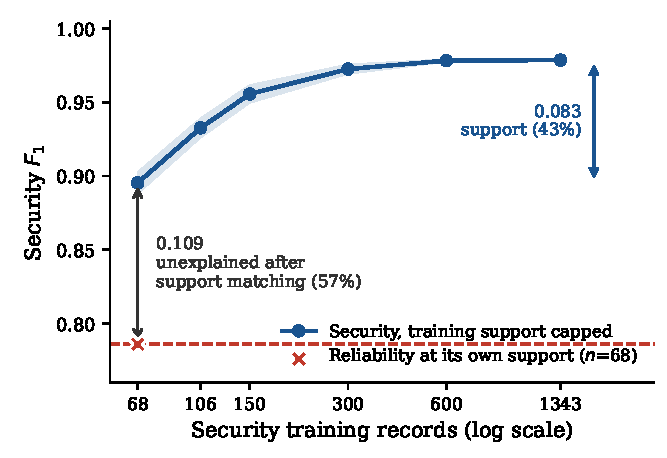
\includegraphics[width=0.70\textwidth]{figures/fig_matched_support.pdf}
\caption{Matched-support experiment. Security's $F_1$ as its training support is capped
(blue, shaded band shows $\pm$1 s.d. over five repeats), against Reliability's $F_1$ at its
own support of 68 records (red). The vertical arrows decompose the 0.193 gap between the two
categories into the part attributable to training-set support and the part that support does not explain.}
\label{fig:matched}
\end{figure}

Figure~\ref{fig:matched} shows why the two must be separated. Had Security's curve descended
to the red line, support would have been a sufficient explanation; had it stayed flat, support
would have been irrelevant. It does neither.

We tested the obvious explanation and can reject it. If Reliability underperformed because its
language is diffuse, it should show a more dispersed vocabulary. At matched support the reverse
holds: it has the lower type--token ratio ($0.286$ against $0.373 \pm 0.014$) and higher
concentration in its twenty commonest terms ($0.488$ against $0.371 \pm 0.013$), and the lowest
vocabulary overlap with other categories (Jaccard 0.258 against 0.272--0.291). It is the most lexically distinct category while remaining the worst classified. The tested
proxies therefore do not support lexical diffuseness as the explanation, which is weaker than
excluding every lexical account.

The error pattern shows an asymmetry toward the majority: 70.5\% of Reliability's false
negatives go to Security, against 14.1\% to Usability and 15.4\% to Performance. This suits
majority-class attraction rather than lexical confusion, but the skew is weaker than the class
prior predicts, and significantly so: against expected shares of 84.0\%, 9.4\% and 6.6\%, a
goodness-of-fit test rejects proportionality ($\chi^2 = 12.56$, df $= 2$, $p = 0.002$).
Majority-class attraction is therefore a partial account. We record the residual as uncharacterised rather
than offer an account the data does not support, and identify it in
Section~\ref{sec:future} as the most tractable open question this study leaves.

A related asymmetry appears in Table~\ref{tab:percat}, where Performance ($n = 106$)
outscores Usability ($n = 150$) for every one of the eight methods despite lower support,
which is a second indication that support alone does not order the categories.

The summary is therefore narrower than the variance decomposition alone would suggest,
and we state it in the narrower form: category dominates method by a wide margin, class support is a demonstrable and substantial component of the category effect, and roughly
half of that effect is something other than support, which we have characterised but not
measured.

\subsection{Training dynamics}
\label{sec:dynamics}

Two properties of the training process bear on how much weight the architectural comparisons
above can carry: whether the models learn the minority categories at all rather than
defaulting to the majority, and how much run-to-run noise checkpoint selection introduces.
Figure~\ref{fig:convergence} plots validation accuracy and macro $F_1$ across epochs for a
representative fold of the full model.

\begin{figure}[htbp]
\centering
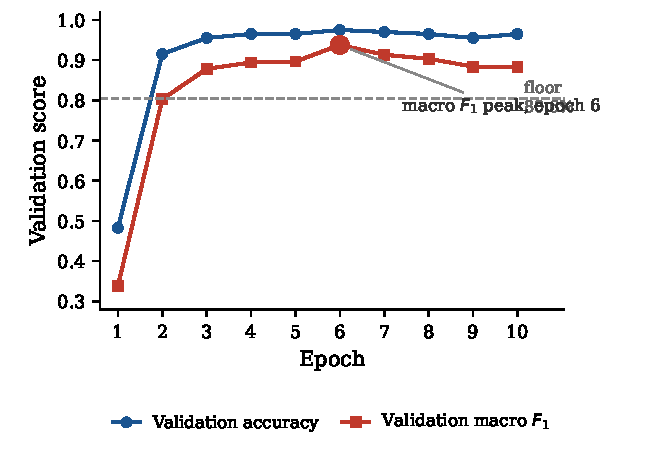
\includegraphics[width=0.70\textwidth]{figures/fig_convergence.pdf}
\caption{Validation accuracy and macro $F_1$ across ten training epochs for the full model
on a representative fold. Accuracy crosses the majority-class floor during the second epoch. Macro $F_1$ peaks at epoch six and then oscillates without systematic improvement.}
\label{fig:convergence}
\end{figure}

Figure~\ref{fig:convergence} confirms two things about the training procedure. The model
learns the minority categories rather than defaulting to the majority: macro $F_1$ rises
from 0.34 to above 0.87 within three epochs, which a majority-class collapse would not
produce. Performance then plateaus by epoch six, after which macro $F_1$ oscillates between
0.88 and 0.94 without systematic gain. The amplitude of that late-epoch oscillation is
comparable to the entire between-configuration spread in Table~\ref{tab:results}, which is
context worth holding when interpreting small architectural differences in this domain: the
noise introduced by checkpoint selection is of the same order as the effects such
comparisons attempt to detect.

% =====================================================================
\section{Discussion}
\label{sec:discussion}

Two questions follow. Whether a null of this kind is informative depends on what the design could have detected and whether the pattern is stable. And what to make of a task on which architecture moves performance so little and labelled-data volume so much. We take these in turn, then set out what follows for research practice and for practitioners.

\subsection{Interpreting the null result}

Our ablation was designed to identify which of several paradigms contributes to NFR
classification, and found that none does at a magnitude the design can resolve. Three
properties support treating this as an informative result rather than an inconclusive one.

The intervals are narrow: each ablation has a 95\% half-width between 0.009 and 0.012 macro
$F_1$, so that no 95\% interval admits a single-component contribution above roughly 0.015 (Table~\ref{tab:equiv}). Gains of two to five points are routinely reported in this literature, and effects of that size would have been detected comfortably.

The result is stable across fold assignments. Configuration ordering changes between repeats rather than settling into a hierarchy, with mean ranks between 3.2 and 4.8 where tied configurations would rank 4.0. This is descriptive: the Friedman test on five blocks is too weak to license an inference either way.

The central result is conditional rather than uniformly negative. Under the fixed four-label protocol none
of the four mechanisms produces a single-component gain the intervals can resolve, and removing all four
leaves an encoder within 0.0018 of Full. Five checks aimed at search budget, source shift, near-duplicate
leakage, contrastive positive-pair availability and graph grounding do not overturn that. The sixth does:
restoring Maintainability and Portability yields $+0.0248$ macro $F_1$ for Full with a conditional interval
above zero. The evidence therefore supports neither a corpus-wide claim that architectural complexity pays
nor one that it does not, but the narrower claim that the comparative value of this composition depends
materially on the label-space definition.

The five protocol analyses ask whether the four-label conclusion survives plausible criticisms. It does, with differing strengths of evidence. They differ in evidential strength but agree in direction. Only the pair-aware contrastive rerun
establishes practical equivalence; the tuning interval is too wide to establish anything; and the source
and grouped analyses place encoder-only ahead on the point estimate while their intervals cross zero.
Together they make a tuning, source-leakage, template-leakage or positive-pair explanation insufficient on
its own to account for the primary null.

In two of the three architectural sensitivities the encoder-only point estimate exceeds the composition's,
and in the third the ordering reverses; all three intervals cross zero. Within the four-label task the
pattern is consistent with no reliable difference rather than a small consistent advantage in either
direction. The six-label sensitivity is the exception, and of a different kind: it does not adjust the protocol but
changes the estimand, which is why it can reverse the ordering without contradicting any protocol check.
The component follow-up then localises the reversal to the graph and contrastive branches, with the
caution that it is exploratory, that its marginal effects sum to 2.7 times the joint effect they are
sometimes assumed to decompose, and that the same GCN ablation is null on four labels.

The design produces a substantially larger point estimate for the classical comparison, approximately
0.025 macro $F_1$, which suggests sensitivity to effects of that approximate magnitude, although this
comparison does not survive familywise correction. The
evaluation is not insensitive; it simply finds no architectural effect.

The finding has precedent. Melis et al.~\cite{melis2018} found a well-tuned LSTM matching the architectures said to have superseded it once search budgets were equalised, and Dacrema et al.~\cite{dacrema2019} found most reproducible neural recommenders beaten by tuned simple baselines. Ours is the same shape reached by a different control: we removed components from one system rather than equalising tuning across many. That independent lines converge suggests the pattern belongs to how architectural claims are evaluated rather than to any one field.

\subsection{Why composition may not help on this task}

Several properties of the task offer plausible explanations, which we distinguish from
demonstrated causes.

The extended-context component has little to operate on. Requirements here are short, with a
median well below the 256-token window, so a mechanism for carrying information across segment
boundaries encounters none. Its removal eliminated 28.9M parameters and 4.6 minutes per fold
while changing macro $F_1$ by 0.0005.

The knowledge graph may duplicate what the encoder already represents. A pre-trained
transformer has encountered \emph{encryption}, \emph{authentication}, \emph{latency} and
\emph{throughput} in context many millions of times, and the relations a hand-built
ISO/IEC 25010 graph makes explicit are plausibly already encoded distributionally. This
reading is worth stating carefully, because injecting domain knowledge into a learned model
is not futile in general. Muhairat et al.~\cite{muhairat2024} mined association rules over a
software engineering curriculum and report that incorporating domain knowledge improved the
accuracy and reliability of their predictions. The difference is that their learner had no
other route to the structure they supplied, whereas ours was initialised from a corpus in
which the same relations are already latent. What our ablation shows is not that structured knowledge is useless for software engineering
tasks, but that on this corpus, under the evaluated implementation and hyperparameter
settings, explicit graph-based domain knowledge did not provide a measurable improvement
beyond the pre-trained encoder.

The task appears substantially lexical. A TF-IDF pipeline reaches 0.873, within 0.026 of every
neural configuration, and recovers 0.895 on Security from 68 training examples. That surface
vocabulary carries most of the achievable signal leaves little headroom for architecture, which
suits how the task was posed: Cleland-Huang et al.~\cite{clelandhuang2007} built their
classifier on indicator terms, and these corpora still largely encode what such terms
identify.

A fourth possibility we cannot exclude: the corpora may impose a ceiling set by label noise and
the single-label formulation rather than by the models, which is what three transformers
converging within 0.0023 would produce. Distinguishing a data ceiling from a modelling limit
needs a human baseline that does not exist (Section~\ref{sec:future}).

\subsection{Where the larger performance differences lie}

Section~\ref{sec:support} reframes what the ablation found. Category accounts for roughly
sixty times as much variance in per-category $F_1$ as method does (91.5\% against 1.5\%),
and spans a range 6.9 times wider. Choice among eight methods spanning classical machine
learning, a bare fine-tuned encoder, an external baseline, and a five-paradigm composition
accounts for 1.5\% of that variance.

The matched-support experiment gives this practical form. A $20\times$ increase in labelled
data for one category moved its $F_1$ by 0.083; the full five-paradigm composition moved
macro $F_1$ by 0.0018 relative to a bare encoder. For a team allocating a fixed budget, the
evidence favours annotation over architecture by a wide margin.

It also explains why two ISO/IEC 25010 categories are absent from our evaluation entirely.
Maintainability and Portability were excluded not because they are intrinsically harder but
because the public corpora contain 34 and 18 labelled examples respectively. No
architecture recovers a category that has not been labelled at sufficient volume, and the
field's shared reliance on these corpora makes this ceiling common to the literature rather
than particular to this study.

\subsection{What a multi-label formulation would change}
Requirements routinely address several quality attributes at once, and our single-label
formulation forces each into one category. The consequence for the ablation is not neutral,
and it cuts in a specific direction. Under single-label scoring, a classifier that
recognises both the security and the reliability content of a replication requirement is
penalised for whichever it does not emit, so the metric cannot reward exactly the kind of
relational reasoning the graph component was added to supply. It is therefore possible that
the GCN contributes something a multi-label metric would detect and ours cannot.

Two observations bound this. The null holds on the majority category too, where cross-cutting
bites least, and the classical baseline recovers most achievable performance without relational
machinery. A multi-label replication is the second most valuable follow-up after the tuning
experiment, and would require re-annotation rather than re-analysis.

\subsection{Implications for research practice}

Reported gains from architectural composition in NFR classification warrant caution until replicated
under controlled conditions. The present study applies five such controls: component ablation on fixed
folds, equal trial budgets, source-holdout evaluation, duplicate-grouped folds and a loss-specific
batching sensitivity. None produces reliable evidence that the composition is superior to the simpler
comparator it is meant to improve upon. Our results do not establish that graph networks,
extended context, contrastive objectives, or meta-learning are without value in
requirements engineering. They establish that on a realistic imbalanced corpus, with folds
and hyperparameters held constant and each component removed in isolation, none contributes
an effect this design can resolve. Studies reporting substantial gains from such components
frequently vary corpus, split, and tuning simultaneously, which cannot separate
architectural contribution from experimental variance.

Four practices would strengthen claims in this area, and we adopt all four. Component-level
ablation on fixed folds isolates architectural contribution. Reporting intervals on
differences, rather than $p$-values alone, distinguishes an absent effect from an
undetected one. Reporting the majority-class floor alongside accuracy prevents imbalanced-corpus results from appearing stronger than they are: on our corpus an unqualified report of ``96\% accuracy'' would overstate the achievement considerably. Per-category support reported alongside per-category $F_1$ exposes where a metric rests on ten predictions rather than a thousand.

A methodological caution follows from Section~\ref{sec:stats}. Pooling paired contingency
counts across repeats of cross-validation inflates test statistics, and in our data it
converts a marginal difference ($p = 0.042$) into an apparently decisive one
($p = 0.002$). Any analysis combining repeated cross-validation with paired significance
testing should treat records, not record-repeat pairs, as the independent units.

\subsection{Implications for practice}

For practitioners the recommendation follows from Table~\ref{tab:results}. A fine-tuned
encoder achieved macro $F_1$ 0.8966 in 4.8 minutes per fold with 82.8M parameters; the full
composition achieved 0.8984 in 10.3 minutes with 116.0M. The simpler model is the
appropriate default, and the additional engineering and computational cost of composition
is not repaid on data of this kind. Where labelling effort is available, it should be
directed at under-represented categories rather than at architecture.

% =====================================================================
\section{Threats to Validity}
\label{sec:threats}

We use the categories of Wohlin et al.~\cite{wohlin2012}, preceded by the limitation bearing
most directly on whether the central result holds.

\paragraph{The absence of hyperparameter search.}
The primary ablation estimates component effects at a common default operating point. The equal-budget
sensitivity of Section~\ref{sec:protocolsens} partially addresses the possibility that the composition is more
tuning-sensitive: both architectures receive 25 inner tuning trials and untouched outer tests. Its
interval $[-0.0152, +0.0337]$ is too wide to exclude a practically meaningful tuned benefit, so the study
cannot claim that exhaustive tuning would never favour composition; conversely the point estimate does not
establish such a benefit either. Late-epoch validation oscillation also remains of the same order as
several architectural contrasts.

Against the concern, the design is symmetric: every configuration received identical treatment,
so the comparison is not biased toward the simpler model. For the concern, composed
architectures may be more hyperparameter-sensitive than single encoders, in which case defaults
penalise them disproportionately. Melis et al.~\cite{melis2018} showed that equalising search
budgets changed which architecture appeared best; their control is the complement of ours, and
neither alone settles the question. The concern is sharpened by work that does optimise: Alhaizaey et al.~\cite{alhaizaey2025}
used Bayesian optimisation and a focal loss for imbalance, and Kurtanović and
Maalej~\cite{kurtanovic2017} used resampling, so our configurations are less adapted to this
task than the literature manages.

We therefore ran the equal-trial-budget experiment rather than leaving it as a proposal
(Section~\ref{sec:protocolsens}). Both architectures received 25 inner tuning trials with the outer test folds
untouched, and the contrast remains indeterminate: $+0.0087$ on an interval of $[-0.0152, +0.0337]$. The
primary null cannot be dismissed as an artefact of tuning only the simple model, but neither can a modest
tuned benefit be excluded, and the fixed-setting result stays conditional on Table~\ref{tab:hyper}.


\paragraph{Construct validity.}
Labels are inherited from the source corpora, so their construct validity is that of
PROMISE, PURE, SecReq, and the Mendeley collection, whose annotation procedures we did not
observe and whose agreement statistics we cannot independently verify. Merging labels
across corpora annotated under different guidelines introduces an inconsistency we did not measure. Our deduplication surfaced one requirement text carrying two labels within the
PROMISE-derived aggregation, which is a lower bound rather than an estimate. Quantifying it would require a manual audit against a single guideline, which we did not
perform. Two indirect indications are available and both are weak. Deduplication surfaced a
single text carrying two labels across the aggregation, which places a floor rather than an
estimate on the inconsistency rate. And the three transformer approaches converge within
0.0023 macro $F_1$, which is the pattern a label ceiling would produce but is equally
consistent with a shared representational limit. An audit of a few hundred records against
one guideline would separate these and would be inexpensive relative to its value. Single-label ground truth also
misrepresents requirements addressing several quality concerns simultaneously, which
Section~\ref{sec:related} notes is the normal case rather than the exception.

\paragraph{Internal validity.}
Fold assignment, seeds, hyperparameters, and class weighting were held constant across
configurations, and each variant was retrained from scratch. We verified programmatically
that no requirement identifier or text appears in both the training and test portion of any
fold, that the knowledge graph is constructed from training data only, and that all pooled
prediction sets cover an identical item set. Measured parameter counts confirm that
architectural ablations took effect. Two residual threats remain. Our ablations remove
components as implemented rather than as conceived, so a different implementation of graph
convolution or meta-learning might contribute where ours does not. And late-epoch
oscillation in validation macro $F_1$ (Figure~\ref{fig:convergence}) is of the same order
as the between-configuration differences, so checkpoint selection contributes noise to every comparison. The five repeats average over this without eliminating it.

\paragraph{Task-definition validity.}
The source material contains six mapped labels, of which the primary task excludes two under the
precision-motivated rule of Section~\ref{sec:corpus}. The completed six-label sensitivity shows this is
consequential: the Full-minus-encoder difference moves from $+0.0018$ to $+0.0248$, with the latter
interval above zero. The primary negative conclusion is therefore not label-space invariant. The six-label
result has its own precision problem, since the restored classes hold 34 and 18 records and 59\% of the
aggregate difference comes from them. The validity boundary is two-sided: the four-label ablation is
cleaner for class-specific precision but changes the task, while the six-label sensitivity preserves the
mapped label space at the cost of weak resolution in its two rarest classes.

\paragraph{External validity.}
Our corpus draws on seven documented collections but is heavily concentrated: one supplies
64.2\% of records and the PROMISE-derived portion only 9.9\% (Table~\ref{tab:provenance}).
Concentration of this degree limits how far the findings generalise, since the properties of
the dominant collection, including its annotation conventions and its class balance,
propagate into every result. Findings should be read as pertaining to this mixture rather
than to NFR classification generally. The encoder is \texttt{distilroberta-base} rather than a full-size model, and a larger encoder might interact differently with the composed components,
though the null result is obtained where headroom for improvement is greatest. All
requirements are in English and the knowledge graph is built from English ISO/IEC 25010
terminology, so multilingual generalisation is untested. Only four of six ISO/IEC 25010
categories carry sufficient data for evaluation, and the corpus comprises 1{,}667
requirements against the tens of thousands typical of industrial projects.

\paragraph{Conclusion validity.}
Our primary inference is a paired bootstrap over records, which addresses both the metric
mismatch and the dependence structure that McNemar's test would mishandle
(Section~\ref{sec:stats}). Five repeats is a modest number for rank-based tests across repeats, which is why the
record-level bootstrap is our sole inferential instrument and why we decline to report
Wilcoxon or Cohen's $d$ at that sample size (Section~\ref{sec:stats}). The transformer advantage over the classical baseline
($p = 0.042$) does not survive Bonferroni correction for the nine comparisons drawn, and we
have described it accordingly rather than as an established effect. A null result is
evidence of absence only within the sensitivity the design achieves. We have therefore reported the excluded effect magnitude (0.015 macro $F_1$ per component at 95\%), together with the
equivalence test that fails at 0.01 and Bayes factors below the conventional threshold for
moderate evidence, rather than resting on
non-significance alone.

% =====================================================================
\section{Limitations and Future Work}
\label{sec:future}

The limitations are ordered by how much each constrains the conclusions: the first three are
properties of the data, the fourth and fifth of our design, and the last a question our results
raise but cannot answer.

\paragraph{Corpus scale, coverage, and independence.}
The binding limitation is the corpus. Four of the six quality labels in the corpus carry enough
labelled data for credible evaluation, the largest outnumbers the smallest twentyfold, and
the corpus is effectively drawn from a single family of sources. Constructing a balanced,
genuinely multi-source NFR corpus, particularly for Maintainability and Portability, is the most valuable contribution available in this area, and our matched-support
experiment indicates it would move performance further than any architectural change we
tested. It requires annotation effort rather than modelling insight.

\paragraph{Absence of a human baseline.}
We cannot say whether macro $F_1$ of 0.898 is close to what the task permits, because no
study has established what trained requirements engineers achieve on the same
classification. Without that reference, no automated result in this literature can be
called sufficient or insufficient for practice. An independent study in which engineers
classify a held-out sample without access to the source annotation guidelines would supply
the ceiling against which every classifier, including ours, should be read.

\paragraph{Single-label formulation.}
Requirements addressing several quality concerns are forced into one category. Multi-label
evaluation would represent the construct more faithfully and change what the per-category
metrics mean. Whether the paradigms we ablated contribute under a multi-label formulation
is untested.

\paragraph{Why the same component behaves differently across label spaces.}
The component follow-up leaves a sharper question than it answers. The GCN ablation is null on four labels
($+0.0029$, interval spanning zero) and resolvable on six ($+0.0225$). Three explanations are consistent
with that: the components may act specifically where labelled data is scarcest; the harder six-label task
may move the comparison away from ceiling so the same mechanism becomes measurable; or the four-label
design may lack the resolution to detect an effect of 0.0225, which sits just beyond the roughly 0.015 it
excludes. Label spaces intermediate between four and six would separate the first two, and an independent
corpus with adequate minority-class support would address the third. Until then the component result
should be read as local to the six-label task.

\paragraph{What the robustness extensions closed.}
Four methodological objections that previously sat in future work are now addressed in the paper itself:
equal-trial-budget tuning (Section~\ref{sec:protocolsens}), neural source-holdout evaluation
(Section~\ref{sec:loso}), near-duplicate-grouped folds (Section~\ref{sec:protocolsens}) and a pair-aware
contrastive sensitivity (Section~\ref{sec:protocolsens}). None reverses the primary conclusion, though the
equal-trial-budget interval remains too wide to exclude a modest tuned benefit. The remaining limitations are
data- and construct-related rather than protocol-related.

\paragraph{Independent, balanced multi-source data.}
Four of the six quality labels have enough data for credible evaluation, the largest evaluated class
outnumbers the smallest nearly twentyfold, and one collection supplies almost two thirds of the records.
The highest-value next contribution is a genuinely independent, multi-organisation corpus with
substantially more Maintainability, Portability, Performance and Reliability examples. The source-holdout
results show that record-level scores should not be assumed to transfer unchanged to a new source, and the
collapse observed on the smallest holdout shows how sharply they can fail.


\paragraph{Component implementations and scale.}
Our ablations remove components as implemented. A different graph construction, a genuine
segment-recurrence mechanism, or second-order MAML might contribute where our versions do not. We have released the implementations so this can be examined rather than assumed.
Whether a full-size encoder interacts differently with the composed components also remains
open.

\paragraph{The residual category effect.}
Roughly 57\% of the Security--Reliability performance gap survives matching on support and
is unexplained. We eliminated the most obvious candidate: lexical diffuseness, which the
measurements in Section~\ref{sec:support} contradict, since Reliability is the more
formulaic and the more lexically distinct of the two. The error pattern instead suggests
majority-class attraction, but weaker than the class prior predicts, so that account is
incomplete. Annotation agreement per category, boundary ambiguity against neighbouring
quality attributes, and controlled paraphrase experiments remain untested and would
sharpen what ``category difficulty'' means here. We regard this as a more promising
direction than further architectural variation.

% =====================================================================
\section{Conclusion}
\label{sec:conclusion}

We asked whether composing multiple learning paradigms improves NFR classification, and
answered with a controlled ablation rather than a headline comparison. Across 175 training
runs, removing the graph convolutional network, the relative-position auxiliary block, the contrastive
objective or the meta-learning stage changes macro $F_1$ by between 0.0001 and 0.0051, and
every interval contains zero. The intervals exclude single-component contributions above
0.015 at the 95\% level. Equivalence at a margin of 0.015 is established for all four
components and at 0.010 for only one, and the Bayes factors fall short of moderate evidence
for the null. A fine-tuned encoder alone matches the full composition at 71\% of the parameters and
47\% of the training time, an independently developed baseline lands within 0.0023 of both,
and even a TF-IDF pipeline is within 0.0254.

The conclusion no longer rests on one random-fold, fixed-default protocol. Equal-trial-budget nested tuning
yields Full 0.9010 against Encoder 0.8923 on an interval crossing zero. Neural leave-one-source-out gives
Full 0.788 against Encoder 0.810 across the three multi-class sources with at least 50 records, and on the
smallest holdout all three neural configurations collapsed to a single predicted label where the classical
pipeline did not. Near-duplicate-grouped folds give Full 0.8754 against Encoder 0.8816. Correcting the
contrastive positive-pair imbalance leaves the two within 0.0003 on an interval inside $\pm 0.01$. None of these five protocol checks reveals a reliable aggregate advantage for the composition on the
four-label task.

The task-definition sensitivity changes that conclusion in an important way. Restoring Maintainability and
Portability gives a 1,719-record six-label task on which Full reaches $0.8286 \pm 0.0113$ against
$0.8038 \pm 0.0088$ for encoder-only, a difference of $+0.0248$ with a 95\% conditional interval of
$[+0.0044, +0.0469]$ that is not compatible with practical equivalence at $\pm 0.01$. The four-label
negative finding does not travel unchanged to the broader label space.

Two qualifications keep that result in proportion. It is not confined to the restored labels: on the four
labels common to both tasks the six-label models differ by $+0.0152$ against $+0.0018$ in the primary
experiment, so what changed is the training problem rather than the set of categories scored. And 59\% of
the aggregate difference comes from two classes holding 34 and 18 records, where the largest single
contribution corresponds to 2.8 additional correct predictions per repeat and reverses sign in one repeat
of five. The strongest available interpretation is therefore not that complexity is generally beneficial or
generally unnecessary, but that task definition materially conditions the comparison.

The component follow-up localises that reversal. Removing the GCN costs 0.0225 macro $F_1$ on the
six-label task and removing the contrastive objective 0.0207, both surviving Holm adjustment across the
four-contrast family; meta-learning and the relative-position block remain unresolved. Three cautions
travel with this. The analysis is exploratory and post-primary. The four marginal effects sum to 0.0671
against a joint effect of 0.0248, so they are marginal removals at the full configuration rather than a
decomposition of the endpoint gap. And the same GCN ablation is null on four labels, so what the follow-up
identifies is a component effect conditional on the label space, not a property of the component.

Where leverage does exist is in the data. Category accounts for 91.5\% of the variation in
per-category $F_1$ against 1.5\% for method, and capping the majority category's training
support at the minority category's level costs 0.083 $F_1$, sixteen times the largest
single-component effect. Support explains 43\% of the gap between those two categories. The residual survives
matching and its causes are not identified by this study; we tested and rejected the natural
lexical explanation for it.

Two properties of the corpus bound all of this. Only four of the six quality labels in the corpus
carry enough labelled data to evaluate, and one class holds 80.6\% of records, so every
accuracy figure must be read against a majority-class floor of 80.56\%. These are properties
of the public NFR datasets rather than of our pipeline.

Our recommendation is methodological. Architectural claims in this area should be accompanied
by component-level ablations on fixed folds, by intervals and a declared smallest effect of
interest rather than $p$-values alone, by majority-class floors reported alongside accuracy,
and by per-category support reported alongside per-category $F_1$. Analyses combining
repeated cross-validation with paired testing should treat records, not record--repeat pairs,
as the independent units: pooling across repeats inflated one of our own comparisons from
$p = 0.042$ to $p = 0.002$. For practitioners, use a fine-tuned encoder and spend the saved
effort on labelling the categories the public corpora leave thin.

% =====================================================================
% Appendix A moved to supplementary material; its three analyses are summarised inline
% in Sections 3.4, 4.5 and 4.10 with full detail in the replication package.

\section*{Declarations}

\paragraph{Data and code availability.}
The corpus, the source spreadsheets, fold assignments, all 175 prediction sets, the
construction, training, and analysis code, the figure-generation scripts, and a verification
script that recomputes every number reported in this paper are archived and citable at
\texttt{[DOI to be inserted on acceptance]}, with a mirror for active maintenance. The verification script exits with a
non-zero status if any reported value disagrees with the released data.

\paragraph{Competing interests.}
The authors declare no competing interests.

\paragraph{Funding.}
This research received no specific grant from any funding agency in the public, commercial,
or not-for-profit sectors.

\paragraph{Author contributions.}
Both authors contributed to the study design, the analysis, and the manuscript.

\paragraph{Use of source data.}
The corpus is derived from publicly available requirements datasets, redistributed under
the terms of their originating collections, which are documented per record in the
replication package.

% =====================================================================
\begin{thebibliography}{99}\small

\bibitem{abad2017} Z. S. H. Abad, O. Karras, P. Ghazi, M. Glinz, G. Ruhe, and K. Schneider.
What works better? A study of classifying requirements. In \emph{IEEE 25th International
Requirements Engineering Conference (RE)}, pages 496--501, 2017.

\bibitem{clelandhuang2007} J. Cleland-Huang, R. Settimi, X. Zou, and P. Solc. Automated
classification of non-functional requirements. \emph{Requirements Engineering}, 2007.

\bibitem{dacrema2019} M. F. Dacrema, P. Cremonesi, and D. Jannach. Are we really making
much progress? A worrying analysis of recent neural recommendation approaches. In
\emph{Proceedings of the 13th ACM Conference on Recommender Systems}, 2019.

\bibitem{dalpiaz2019} F. Dalpiaz, D. Dell'Anna, F. B. Aydemir, and S. Çevikol.
Requirements classification with interpretable machine learning and dependency parsing. In
\emph{IEEE 27th International Requirements Engineering Conference (RE)}, 2019.

\bibitem{demsar2006} J. Demšar. Statistical comparisons of classifiers over multiple data
sets. \emph{Journal of Machine Learning Research}, 7:1--30, 2006.

\bibitem{devlin2019} J. Devlin, M.-W. Chang, K. Lee, and K. Toutanova. BERT: Pre-training
of deep bidirectional transformers for language understanding. In \emph{Proceedings of
NAACL-HLT}, pages 4171--4186, 2019.

\bibitem{dietterich1998} T. G. Dietterich. Approximate statistical tests for comparing
supervised classification learning algorithms. \emph{Neural Computation},
10(7):1895--1923, 1998.

\bibitem{iipinge2023} V. J. Iipinge, M. Zhang, and Y. Wang. Automated methodology for
classifying non-functional requirements: challenges, validation aspects and new research
directions. In \emph{9th International Conference on Computing and Artificial Intelligence},
2023.

\bibitem{ferrari2017} A. Ferrari, G. O. Spagnolo, and S. Gnesi. PURE: A dataset of public
requirements documents. In \emph{IEEE 25th International Requirements Engineering
Conference (RE)}, 2017.

\bibitem{he2009} H. He and E. A. Garcia. Learning from imbalanced data. \emph{IEEE
Transactions on Knowledge and Data Engineering}, 21(9):1263--1284, 2009.

\bibitem{kipf2017} T. N. Kipf and M. Welling. Semi-supervised classification with graph
convolutional networks. In \emph{International Conference on Learning Representations},
2017.

\bibitem{knauss2011} E. Knauss, S. Houmb, K. Schneider, S. Islam, and J. Jürjens.
Supporting requirements engineers in recognising security issues. In \emph{Requirements
Engineering: Foundation for Software Quality (REFSQ)}, 2011.

\bibitem{kurtanovic2017} Z. Kurtanović and W. Maalej. Automatically classifying functional
and non-functional requirements. In \emph{IEEE 25th International Requirements Engineering
Conference (RE)}, 2017.

\bibitem{lipton2019} Z. C. Lipton and J. Steinhardt. Troubling trends in machine learning
scholarship. \emph{Queue}, 17(1), 2019.

\bibitem{lessmann2008} S. Lessmann, B. Baesens, C. Mues, and S. Pietsch. Benchmarking
classification models for software defect prediction: a proposed framework and novel findings.
\emph{IEEE Transactions on Software Engineering}, 34(4):485--496, 2008.

\bibitem{li2022} B. Li and C. Nong. Automatically classifying non-functional requirements using
deep neural network. \emph{Pattern Recognition}, 132:108948, 2022.

\bibitem{liu2019roberta} Y. Liu, M. Ott, N. Goyal, J. Du, M. Joshi, D. Chen, O. Levy,
M. Lewis, L. Zettlemoyer, and V. Stoyanov. RoBERTa: A robustly optimized BERT pretraining
approach. \emph{arXiv:1907.11692}, 2019.

\bibitem{melis2018} G. Melis, C. Dyer, and P. Blunsom. On the state of the art of
evaluation in neural language models. In \emph{International Conference on Learning
Representations}, 2018.

\bibitem{reimers2017} N. Reimers and I. Gurevych. Reporting score distributions makes a
difference: Performance study of LSTM-networks for sequence tagging. In \emph{Proceedings of EMNLP}, 2017.

\bibitem{sanh2019} V. Sanh, L. Debut, J. Chaumond, and T. Wolf. DistilBERT, a distilled
version of BERT: smaller, faster, cheaper and lighter. \emph{arXiv:1910.01108}, 2019.

\bibitem{winkler2016} J. Winkler and A. Vogelsang. Automatic classification of
requirements based on convolutional neural networks. In \emph{IEEE 24th International
Requirements Engineering Conference Workshops (REW)}, 2016.

\bibitem{wohlin2012} C. Wohlin, P. Runeson, M. Höst, M. C. Ohlsson, B. Regnell, and
A. Wesslén. \emph{Experimentation in Software Engineering}. Springer, 2012.

\bibitem{alhaizaey2025} A. Alhaizaey, J. Al-Jaroodi, and N. Mohamed. Automated classification
and identification of non-functional requirements in agile-based requirements using pre-trained
language models. \emph{IEEE Access}, 2025.

\bibitem{althunibat2025} A. Althunibat. A quality-focused evaluation framework of customer
satisfaction for mobile services application: a case study from Jordan. \emph{International
Journal of Advances in Soft Computing and its Applications}, 2025.

\bibitem{baker2019} C. Baker, L. Deng, S. Chakraborty, and J. Dehlinger. Automatic multi-class
non-functional software requirements classification using neural networks. In \emph{IEEE 43rd
Annual Computer Software and Applications Conference (COMPSAC)}, 2019.

\bibitem{canedo2020} E. D. Canedo and B. C. Mendes. Software requirements classification
using machine learning algorithms. \emph{Entropy}, 22(9):1057, 2020.

\bibitem{casamayor2010} A. Casamayor, D. Godoy, and M. Campo. Identification of
non-functional requirements in textual specifications: A semi-supervised learning approach.
\emph{Information and Software Technology}, 52(4):436--445, 2010.

\bibitem{chen2025} S. Chen, Y. Zheng, D. Lin, P. Cai, Y. Xiao, and S. Wang.
MAML-KalmanNet: A neural network-assisted Kalman filter based on model-agnostic
meta-learning. \emph{IEEE Transactions on Signal Processing}, 2025.
  \newblock DOI: 10.1109/TSP.2025.3540018.

\bibitem{chung2000} L. Chung, B. A. Nixon, E. Yu, and J. Mylopoulos. Softgoal
interdependency graphs. In \emph{Non-Functional Requirements in Software Engineering},
pages 47--88. Springer, 2000.

\bibitem{chung2012} L. Chung, B. A. Nixon, E. Yu, and J. Mylopoulos.
\emph{Non-Functional Requirements in Software Engineering}, volume 5. Springer, 2012.

\bibitem{dacrema2021} M. Ferrari Dacrema, S. Boglio, P. Cremonesi, and D. Jannach. A troubling
analysis of reproducibility and progress in recommender systems research. \emph{ACM Transactions
on Information Systems}, 39(2), 2021.

\bibitem{dai2019} Z. Dai, Z. Yang, Y. Yang, J. Carbonell, Q. V. Le, and R. Salakhutdinov.
Transformer-XL: Attentive language models beyond a fixed-length context.
\emph{arXiv:1901.02860}, 2019.

\bibitem{dellanna2023} D. Dell'Anna, F. B. Aydemir, and F. Dalpiaz. Evaluating classifiers
in SE research: the ECSER pipeline and two replication studies. \emph{Empirical Software
Engineering}, 28(1):3, 2022.

\bibitem{finn2017} C. Finn, P. Abbeel, and S. Levine. Model-agnostic meta-learning for fast
adaptation of deep networks. In \emph{International Conference on Machine Learning}, pages
1126--1135, 2017.

\bibitem{firesmith2003} D. Firesmith. Engineering security requirements. \emph{Journal of
Object Technology}, 2(1):53--68, 2003.

\bibitem{glinz2007} M. Glinz. On non-functional requirements. In \emph{15th IEEE
International Requirements Engineering Conference (RE)}, pages 21--26, 2007.

\bibitem{haque2019} M. A. Haque, M. A. Rahman, and M. S. Siddik. Non-functional
requirements classification with feature extraction and machine learning: An empirical
study. In \emph{1st International Conference on Advances in Science, Engineering and
Robotics Technology (ICASERT)}, pages 1--5, 2019.
  \newblock DOI: 10.1109/ICASERT.2019.8934499.

\bibitem{hey2020} T. Hey, J. Keim, A. Koziolek, and W. F. Tichy. NoRBERT: Transfer learning
for requirements classification. In \emph{IEEE 28th International Requirements Engineering
Conference (RE)}, pages 169--179, 2020.

\bibitem{hussain2016} A. Hussain, E. O. C. Mkpojiogu, and F. Mohmad Kamal. The role of
requirements in the success or failure of software projects. \emph{International Review of
Management and Marketing}, 6(S7):306--311, 2016.

\bibitem{iso25010} International Organization for Standardization. Systems and software
engineering --- Systems and software Quality Requirements and Evaluation (SQuaRE) ---
System and software quality models. ISO/IEC 25010:2011, 2011.

\bibitem{iso29148} ISO/IEC/IEEE. Systems and software engineering --- Life cycle processes
--- Requirements engineering. ISO/IEC/IEEE 29148:2018, 2018.

\bibitem{kaur2024} K. Kaur and P. Kaur. The application of AI techniques in requirements
classification: a systematic mapping. \emph{Artificial Intelligence Review}, 57:57, 2024.

\bibitem{khosla2020} P. Khosla, P. Teterwak, C. Wang, A. Sarna, Y. Tian, P. Isola,
A. Maschinot, C. Liu, and D. Krishnan. Supervised contrastive learning. \emph{Advances in
Neural Information Processing Systems}, 33:18661--18673, 2020.

\bibitem{liu2022} Z. Liu and J. Zhou. \emph{Introduction to Graph Neural Networks}.
Springer Nature, 2022.

\bibitem{rahimi2021} N. Rahimi, F. Eassa, and L. Elrefaei. One- and two-phase software
requirement classification using ensemble deep learning. \emph{Entropy}, 23(10):1264, 2021.

\bibitem{rahman2023} A. Rahman, M. S. Siddik, and others. Non-functional requirements
classification using machine learning algorithms. \emph{International Journal of Intelligent
Systems and Applications}, 2023.

\bibitem{muhairat2024} M. I. Muhairat, S. Bani-Mohammad, and others. Leveraging machine
learning for predictive pathways in higher education: a case study at Al-Zaytoonah
University of Jordan. \emph{International Journal of Electronics and Communication
Engineering}, 2024.

\bibitem{ralph2020} P. Ralph, N. bin Ali, S. Baltes, D. Bianculli, J. Diaz, Y. Dittrich,
N. Ernst, M. Felderer, R. Feldt, A. Filieri, et al. Empirical standards for software
engineering research. \emph{arXiv:2010.03525}, 2020.

\bibitem{rouder2009} J. N. Rouder, P. L. Speckman, D. Sun, R. D. Morey, and G. Iverson.
Bayesian $t$ tests for accepting and rejecting the null hypothesis. \emph{Psychonomic
Bulletin and Review}, 16(2):225--237, 2009.

\bibitem{saleem2025} M. B. Saleem, N. Qamar, R. Danial, K. Sardar, M. Noor, and U. Omer.
Analyzing the impact of machine learning algorithms on software requirements classification.
\emph{VFAST Transactions on Software Engineering}, 13(1):88--98, 2025.

\bibitem{shafikuzzaman2025} M. Shafikuzzaman, M. R. Islam, S. Zaman, A. Ma, and
A. I. Sifat. On the effectiveness of zero-shot and few-shot pretrained language models for
software requirement classification. \emph{IEEE Access}, 2025.

\bibitem{slankas2013} J. Slankas and L. Williams. Automated extraction of non-functional
requirements in available documentation. In \emph{1st International Workshop on Natural
Language Analysis in Software Engineering (NaturaLiSE)}, pages 9--16, 2013.

\bibitem{song2021} X. Song, R. Ma, J. Li, M. Zhang, and D. P. Wipf. Network in graph neural
network. \emph{arXiv:2111.11638}, 2021.

\bibitem{subahi2023} A. F. Subahi. BERT-based approach for greening software requirements
engineering through non-functional requirements. \emph{IEEE Access}, 11:103001--103013,
2023.
  \newblock DOI: 10.1109/ACCESS.2023.3317798.

\bibitem{vaswani2017} A. Vaswani, N. Shazeer, N. Parmar, J. Uszkoreit, L. Jones,
A. N. Gomez, {\L}. Kaiser, and I. Polosukhin. Attention is all you need. \emph{Advances in
Neural Information Processing Systems}, 30, 2017.

\end{thebibliography}

\end{document}
